%%%%%%%%%%%%%%%%%%%%%%%%%%%%%%%%%%%%%%%%%
% Kaggle Assignment
% LaTeX Template
% 
%%%%%%%%%%%%%%%%%%%%%%%%%%%%%%%%%%%%%%%%%

%----------------------------------------------------------------------------------------
%	PACKAGES AND OTHER DOCUMENT CONFIGURATIONS
%----------------------------------------------------------------------------------------

\documentclass[11pt]{scrartcl} % Font size

%%%%%%%%%%%%%%%%%%%%%%%%%%%%%%%%%%%%%%%%%
% Wenneker Assignment
% Structure Specification File
% Version 2.0 (12/1/2019)
%
% This template originates from:
% http://www.LaTeXTemplates.com
%
% Authors:
% Vel (vel@LaTeXTemplates.com)
% Frits Wenneker
%
% License:
% CC BY-NC-SA 3.0 (http://creativecommons.org/licenses/by-nc-sa/3.0/)
% 
%%%%%%%%%%%%%%%%%%%%%%%%%%%%%%%%%%%%%%%%%

%----------------------------------------------------------------------------------------
%	PACKAGES AND OTHER DOCUMENT CONFIGURATIONS
%----------------------------------------------------------------------------------------

\usepackage{amsmath, amsfonts, amsthm} % Math packages

\usepackage{listings} % Code listings, with syntax highlighting

\usepackage[english]{babel} % English language hyphenation

\usepackage{graphicx} % Required for inserting images
\graphicspath{{../graphics/}{./}} % Specifies where to look for included images (trailing slash required)

\usepackage{booktabs} % Required for better horizontal rules in tables

\numberwithin{equation}{section} % Number equations within sections (i.e. 1.1, 1.2, 2.1, 2.2 instead of 1, 2, 3, 4)
\numberwithin{figure}{section} % Number figures within sections (i.e. 1.1, 1.2, 2.1, 2.2 instead of 1, 2, 3, 4)
\numberwithin{table}{section} % Number tables within sections (i.e. 1.1, 1.2, 2.1, 2.2 instead of 1, 2, 3, 4)

\setlength\parindent{0pt} % Removes all indentation from paragraphs

\usepackage{enumitem} % Required for list customisation
\setlist{noitemsep} % No spacing between list items

\usepackage{tikz}
\usetikzlibrary{arrows, positioning, automata}
\usepackage{amsfonts}
\usepackage{multirow}
\usepackage{hyperref}

%----------------------------------------------------------------------------------------
%	DOCUMENT MARGINS
%----------------------------------------------------------------------------------------

\usepackage{geometry} % Required for adjusting page dimensions and margins

\geometry{
	paper=a4paper, % Paper size, change to letterpaper for US letter size
	top=2.5cm, % Top margin
	bottom=3cm, % Bottom margin
	left=3cm, % Left margin
	right=3cm, % Right margin
	headheight=0.75cm, % Header height
	footskip=1.5cm, % Space from the bottom margin to the baseline of the footer
	headsep=0.75cm, % Space from the top margin to the baseline of the header
	%showframe, % Uncomment to show how the type block is set on the page
}

%----------------------------------------------------------------------------------------
%	FONTS
%----------------------------------------------------------------------------------------

\usepackage[utf8]{inputenc} % Required for inputting international characters
\usepackage[T1]{fontenc} % Use 8-bit encoding

\usepackage{fourier} % Use the Adobe Utopia font for the document

%----------------------------------------------------------------------------------------
%	SECTION TITLES
%----------------------------------------------------------------------------------------

\usepackage{sectsty} % Allows customising section commands

\sectionfont{\vspace{6pt}\centering\normalfont\scshape} % \section{} styling
\subsectionfont{\normalfont\bfseries} % \subsection{} styling
\subsubsectionfont{\normalfont\itshape} % \subsubsection{} styling
\paragraphfont{\normalfont\scshape} % \paragraph{} styling

%----------------------------------------------------------------------------------------
%	HEADERS AND FOOTERS
%----------------------------------------------------------------------------------------

\usepackage{scrlayer-scrpage} % Required for customising headers and footers

\ohead*{} % Right header
\ihead*{} % Left header
\chead*{} % Centre header

\ofoot*{} % Right footer
\ifoot*{} % Left footer
\cfoot*{\pagemark} % Centre footer
 % Include the file specifying the document structure and custom commands

%----------------------------------------------------------------------------------------
%	TITLE SECTION
%----------------------------------------------------------------------------------------

\title{	
	\normalfont\normalsize
	\textsc{Southern Methodist University\\
	 MSDS 6371(401)}\\ % Your university, school and/or department name(s)
	\vspace{25pt} % Whitespace
	\rule{\linewidth}{0.5pt}\\ % Thin top horizontal rule
	\vspace{20pt} % Whitespace
	{\huge Kaggle Project}\\ % The assignment title
	\vspace{12pt} % Whitespace
	\rule{\linewidth}{2pt}\\ % Thick bottom horizontal rule
	\vspace{12pt} % Whitespace
}

\author{\LARGE Michael J Wolfe\\
			\LARGE Sandesh Ojha\\
			\LARGE Carl Walenciak\\
			\LARGE Travis Daun\\
			\\
			\small \href{https://github.com/mjwolfe91/SFDS_401_Team3_Kaggle_Project}{Github Repository}\\
			\small \href{https://github.com/mjwolfe91/SFDS_401_Team3_Kaggle_Project}{https://github.com/mjwolfe91/SFDS\_401\_Team3\_Kaggle\_Project}\\} % Your name

\date{\normalsize\today} % Today's date (\today) or a custom date

\newcommand{\STAB}[1]{\begin{tabular}{@{}c@{}}#1\end{tabular}}

\begin{document}

\maketitle % Print the title


\pagebreak

%------------------------------------------------

\tableofcontents{}
\pagebreak
%------------------------------------------------


\section{Introduction}
\paragraph{} Many factors can impact the sale price of residential real estate. This report will explore those various aspects to help define what factors tend to impact home prices. We start by looking at the three distinct neighborhoods (North Ames, Edwards, and Brookside) in Ames, Iowa that Century 21 Ames sells houses to help better understand how above ground living space relates to sales price in each of these neighborhoods and if the neighborhood has an impact on the sales price. At the conclusion of this analysis, we provide a conclusion that quantifies the relationship between living area and sales price with respect to these neighborhoods.
\paragraph{} After examining the impact of above ground living space on sales price for these three neighborhoods, we provide a much more complex analysis of factors that can be used to determine sales price for Ames as a whole. While we will use various methods to determine what factors are important for our predictive model, we will test this model on a blind dataset to show how it performs. The results of this model on the test data will be provided to further build the level of confidence in this tool for predicting future home sale prices.
%------------------------------------------------

\section{Data Description}
The dataset used for this analysis was retrieved from \href{https://www.kaggle.com/c/house-prices-advanced-regression-techniques}{www.kaggle.com/c/house-prices-advanced-regression-techniques}.
\paragraph{Data} The data for this evaluation contained 79 explanatory variables describing (almost) every aspect of residential homes in Ames, Iowa. A complete description of these data can be found in Appendix ~\ref{sec:DataDescription}. The explanatory variables contain both categorical and numeric attributes.  Appendix~\ref{tab:Data}, provides a high level summary of the variables and variable types contained in this dataset.
\paragraph{Preprocessing} The variable \texttt{LotFrontage} posed a challenge since it was a continuous numerical variable that contained \texttt{NA}. This is because the variable was for the linear feet of street connected to property. In many cases (259 of 1460) this was either unknown or unrecorded. Our team made the decision to convert these NA values to 0. We believe this is an acceptable practice since we performed a sensitivity analysis by replacing the NAs with values from 0 to 140 (mean value is 70) with no impact on the linear regression model selection process and this factor was not utilized in any of our final models.
\paragraph{Training} Training of the linear regression models will be done utilizing the \texttt{training.csv} data obtained from above. A five fold cross validation will be employed for model selection. 
\paragraph{Testing} Testing of the linear regression models will be done utilizing the \texttt{test.csv} data obtained from above.
\paragraph{Results} Datafiles containing the test results of the linear regression models can be found in our Github repository at \href{https://github.com/mjwolfe91/SFDS_401_Team3_Kaggle_Project}{https://github.com/mjwolfe91/SFDS\_401\_Team3\_Kaggle\_Project}\\
			




%------------------------------------------------

\section{Analysis Question 1}
\subsection{Restatement of Problem}
\paragraph{Request} Century 21 Ames only sells houses in the Noth Ames, Edwards and Brookside neighborhoods and wants an estimate of how the sale price of the house is related to the square footage of the living area of the house. Additionally, Century 21 Ames would like to know if the sale price (and its relationship to square footage) depends on which neighborhood the house is located in. A fit a model will be used to answer this question.
\paragraph{Deliverable} Provide the estimate (or estimates if it varies by neighborhood) as well as confidence intervals for any estimate(s) you provide. Provide evidence that the model assumptions are met and that any suspicious observations (outliers / influential observations) have been identified and addressed. Finally, a conclusion that quantifies the relationship between living area and sale price with respect to these three neighborhoods.
\subsection{Build and Fit the Model}
\paragraph{} Appendix~\ref{sec:Analysis1}{. Source Code For Analysis 1} contains the SAS code used to check the assumptions, clean the data, and run the model to determine the best estimate for sale price based on square footage for the North Ames, Edwards, and Brookside neighborhoods. We removed four data points from the original dataset due to being outliers. First sale prices greater than \$300,000 were determined to not be representative of the total population of these three neighborhoods. Second, sale condition was limited to only those that were normal sales. Again we feel that home sales that were not normal sales such as foreclosures, linked properties, and land purchases were not representative of the population of interest.
\begin{figure}[h] % [h] forces the figure to be output where it is defined in the code (it suppresses floating)
	\centering
	\begin{tabular}{p{0.48\textwidth} p{0.48\textwidth}}
	\hline
	\multicolumn{1}{|c|}{Original} & \multicolumn{1}{|c|}{After Removal of Outliers} \\
		\multicolumn{1}{|c|}{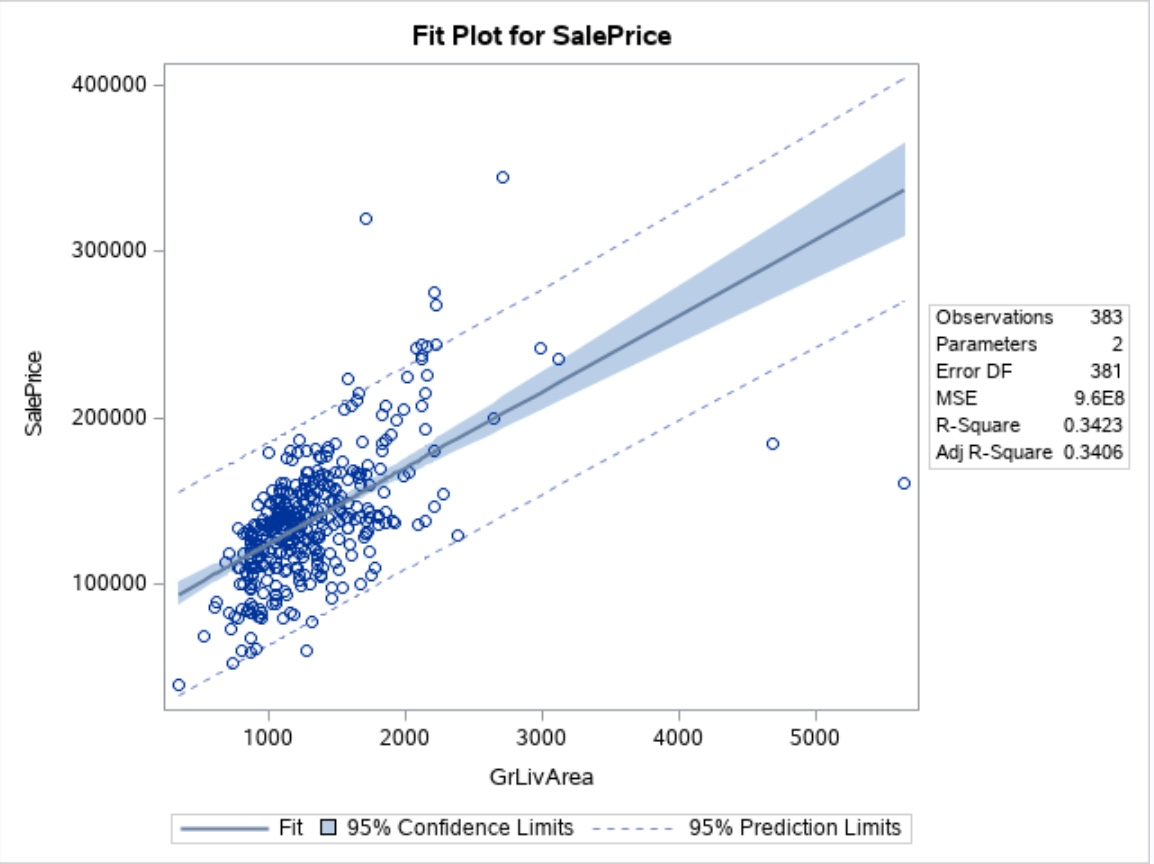
\includegraphics[width=0.48\textwidth]{../graphics/A1LR1}} &
		\multicolumn{1}{|c|}{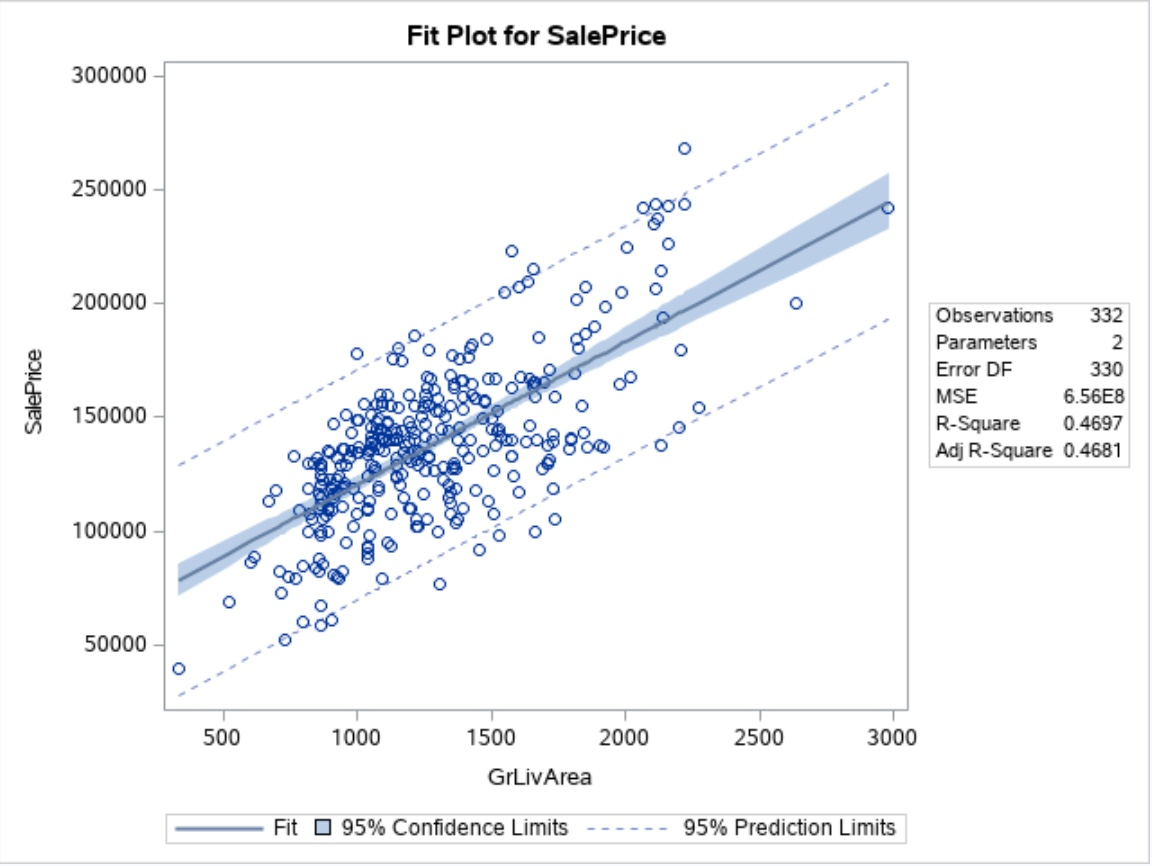
\includegraphics[width=0.48\textwidth]{../graphics/A1LR2}}\\
		\hline
	\end{tabular}		
	\caption{Simple Linear Regression Models.}
	\label{fig:A1LR}
\end{figure}
%------------------------------------------------

\subsection{Checking Assumptions}
\begin{figure}[h] % [h] forces the figure to be output where it is defined in the code (it suppresses floating)
	\centering
	\begin{tabular}{p{0.23\textwidth} p{0.23\textwidth}p{0.23\textwidth}p{0.23\textwidth}}
\hline	
	\multicolumn{2}{|c|}{Original} &  \multicolumn{2}{|c|}{After Removal of Outliers} \\
		\multicolumn{1}{|c}{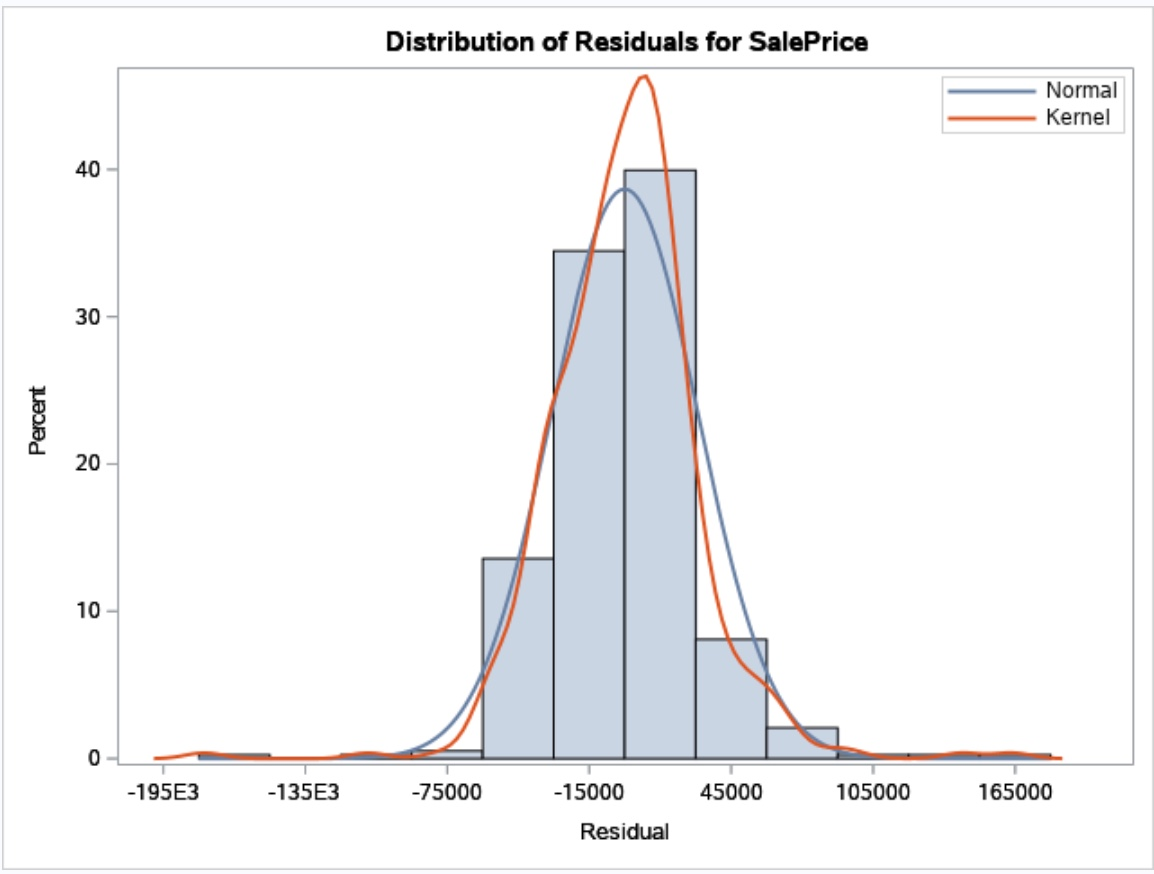
\includegraphics[width=0.23\textwidth]{../graphics/A1Norm1}} &
		\multicolumn{1}{c|}{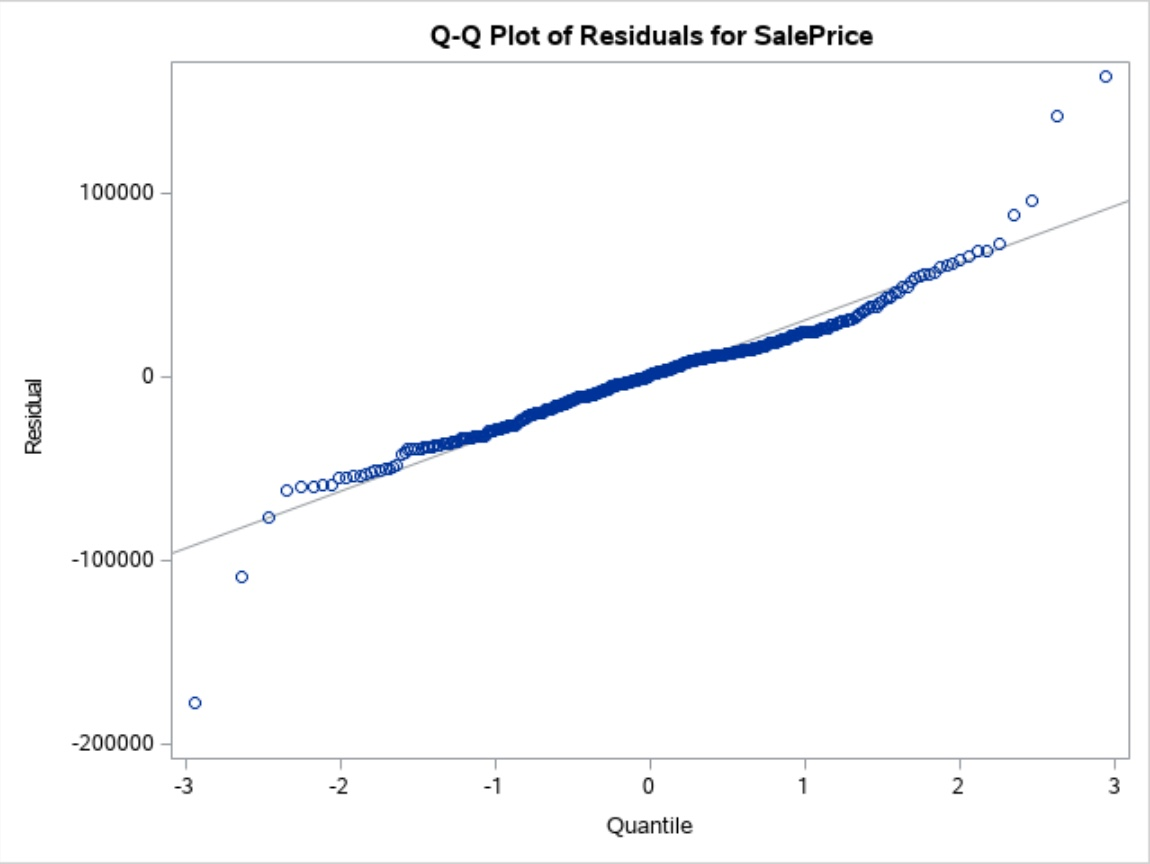
\includegraphics[width=0.23\textwidth]{../graphics/A1qq1}} &
		\multicolumn{1}{|c}{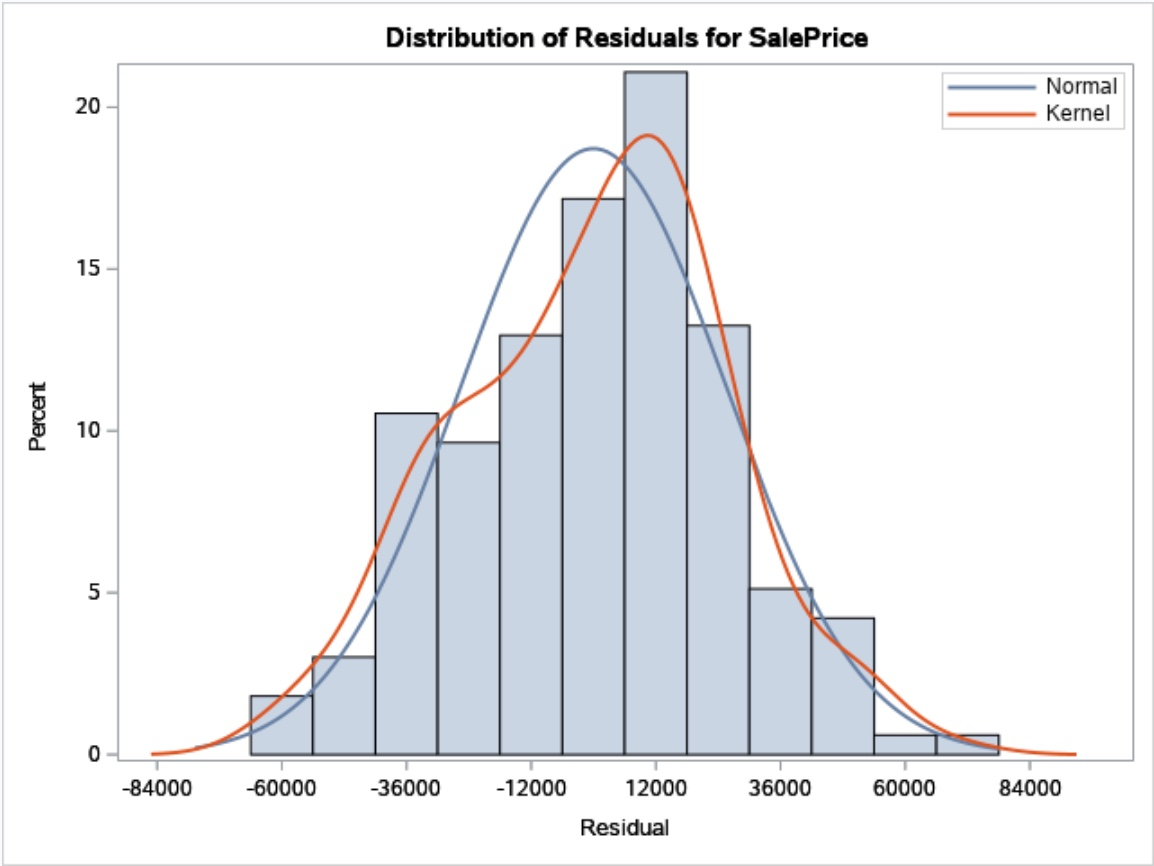
\includegraphics[width=0.23\textwidth]{../graphics/A1Norm2}} &
		\multicolumn{1}{c|}{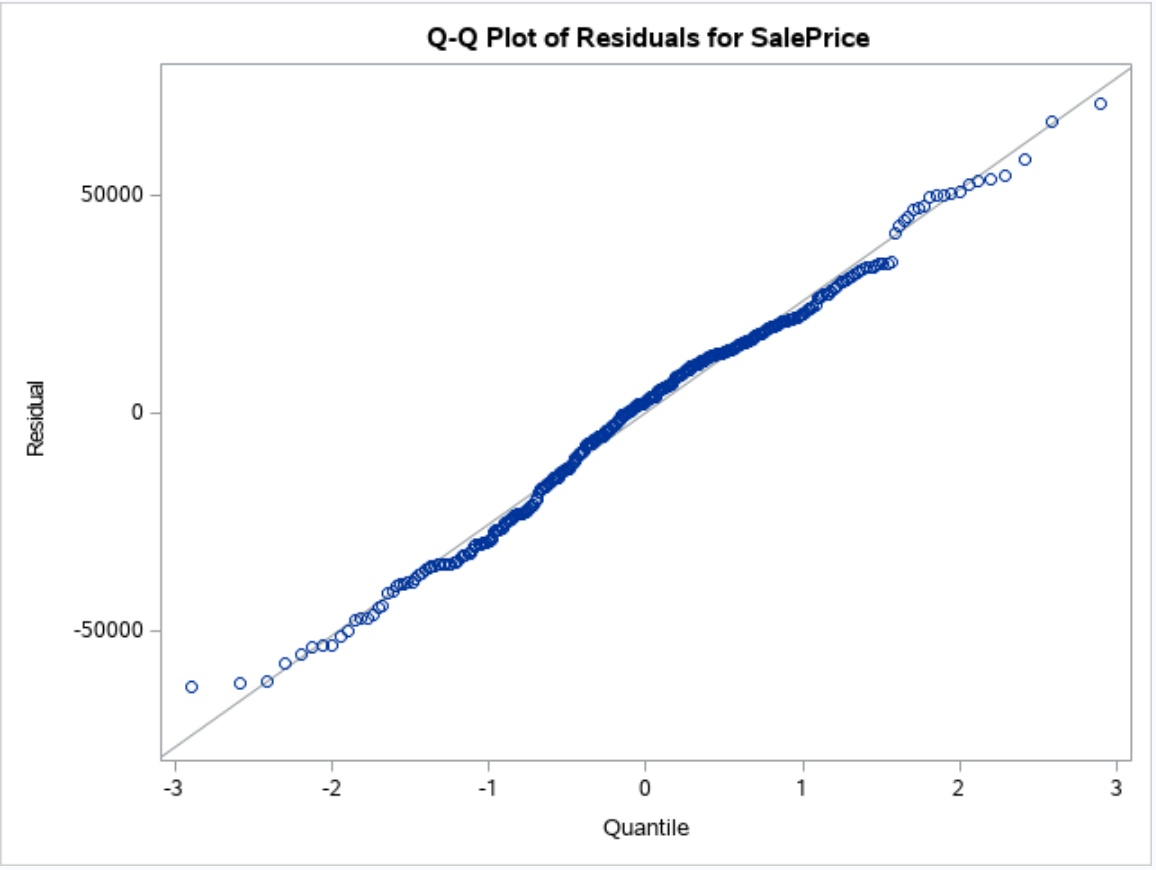
\includegraphics[width=0.23\textwidth]{../graphics/A1qq2}}\\
		\hline
	\end{tabular}		
	\caption{Normality Plots.}
	\label{fig:A1QQ}
\end{figure}

\begin{figure}[h] % [h] forces the figure to be output where it is defined in the code (it suppresses floating)
	\centering
	\begin{tabular}{p{0.23\textwidth} p{0.23\textwidth}p{0.23\textwidth}p{0.23\textwidth}}
	\hline
	\multicolumn{2}{|c|}{Original} &  \multicolumn{2}{|c|}{After Removal of Outliers} \\
		\multicolumn{1}{|c}{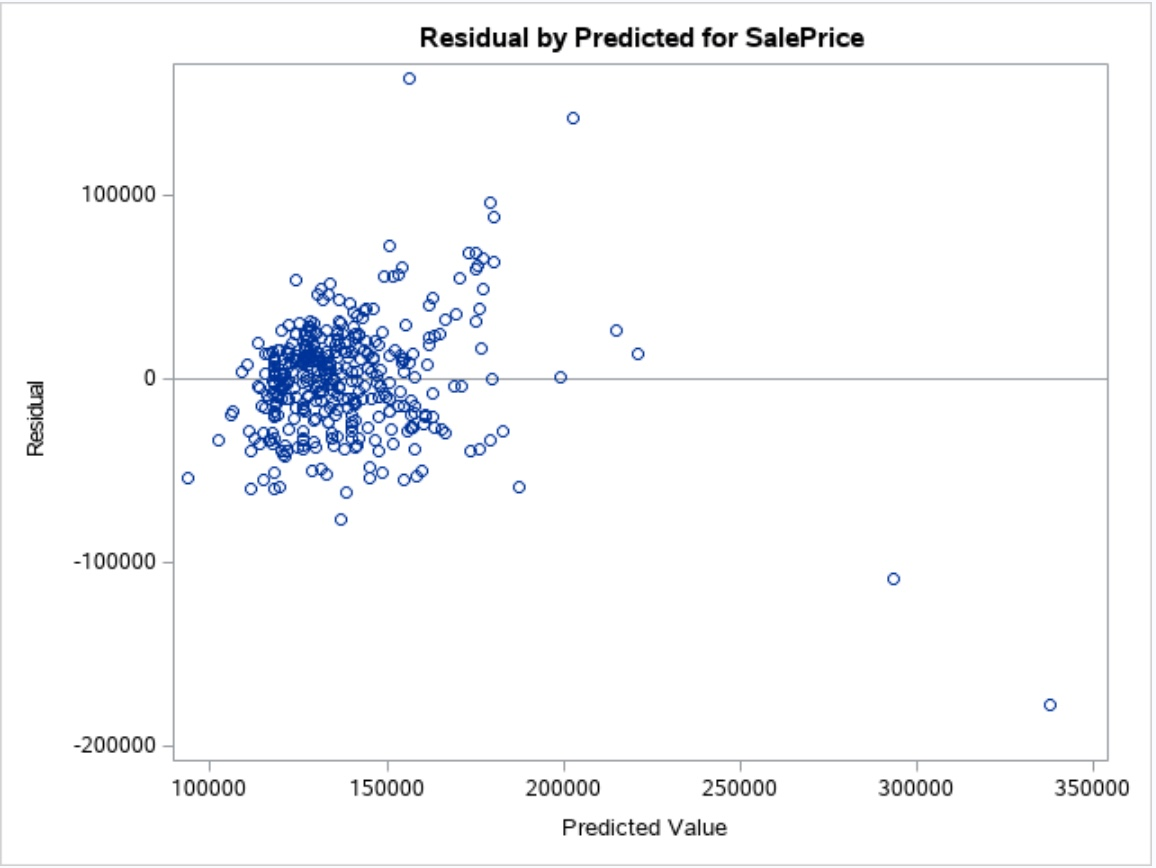
\includegraphics[width=0.23\textwidth]{../graphics/A1Residuals1}} &
		\multicolumn{1}{c|}{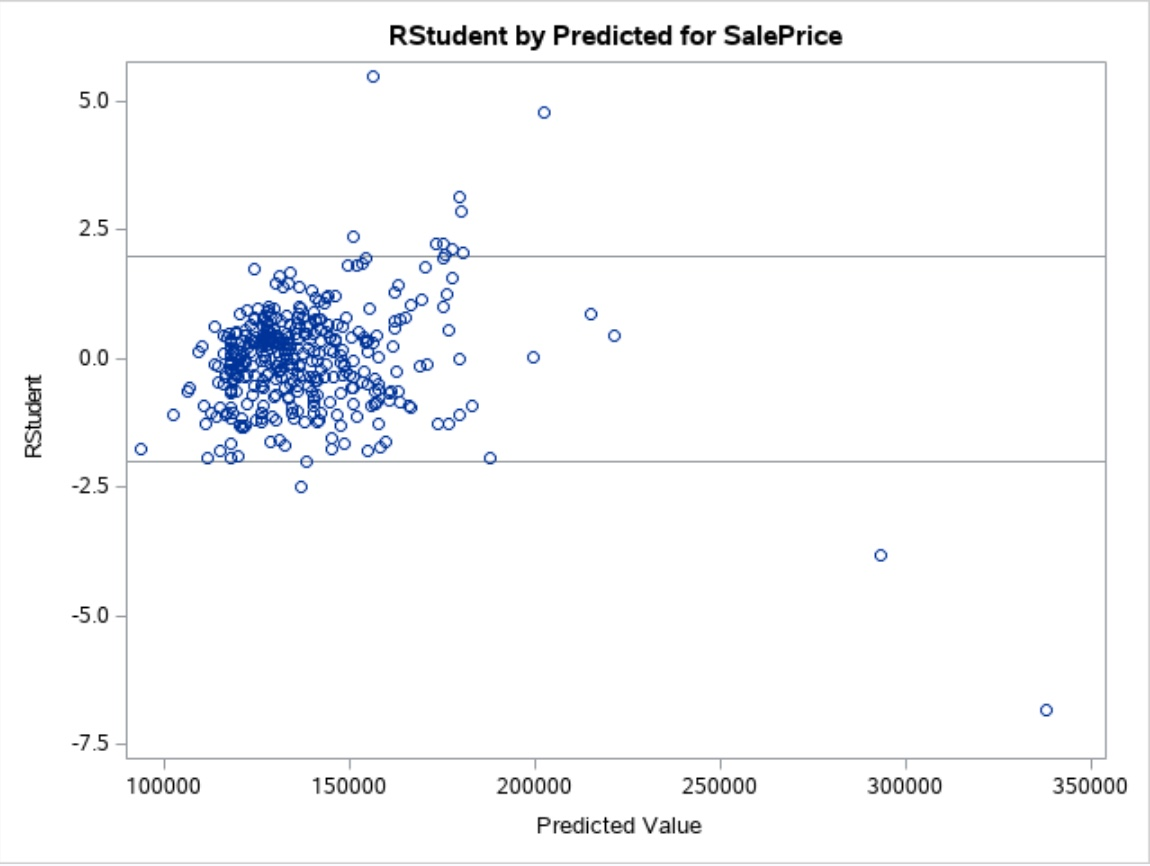
\includegraphics[width=0.23\textwidth]{../graphics/A1StudentResiduals1}} &
		\multicolumn{1}{|c}{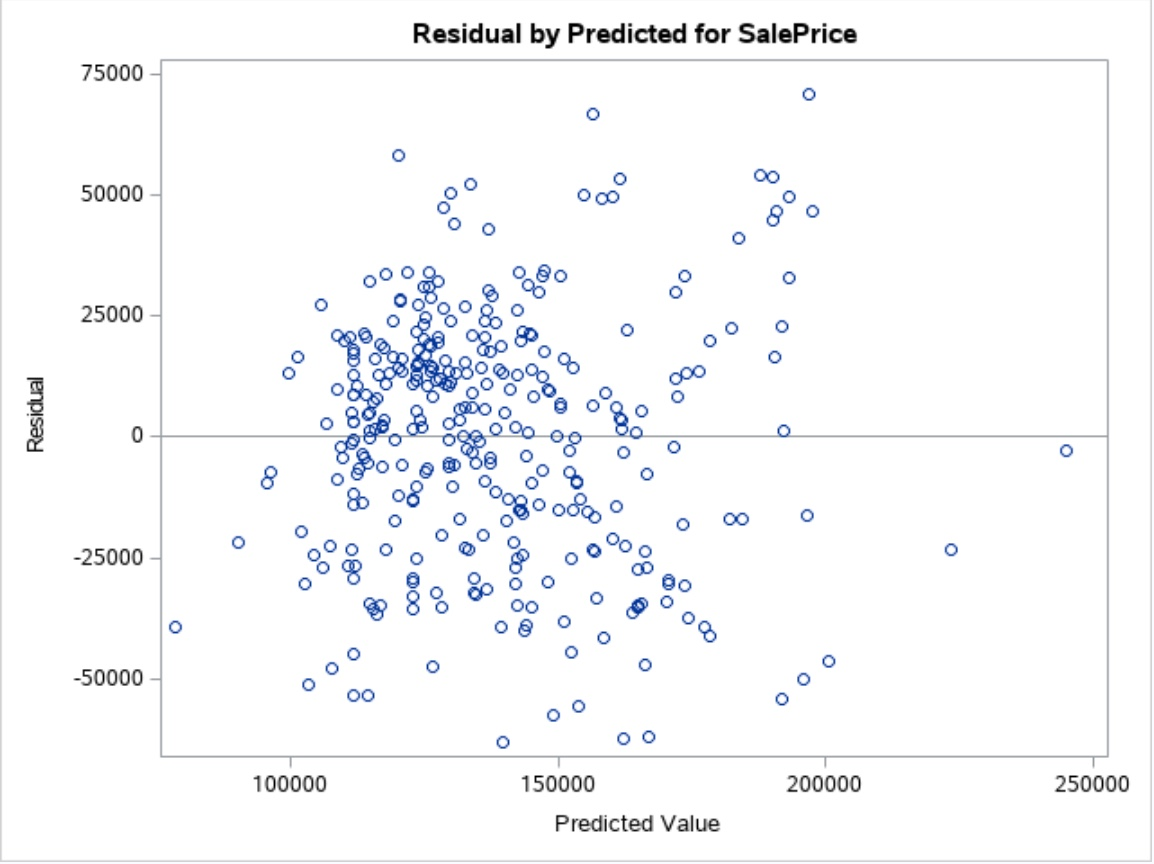
\includegraphics[width=0.23\textwidth]{../graphics/A1Residuals2}} &
		\multicolumn{1}{c|}{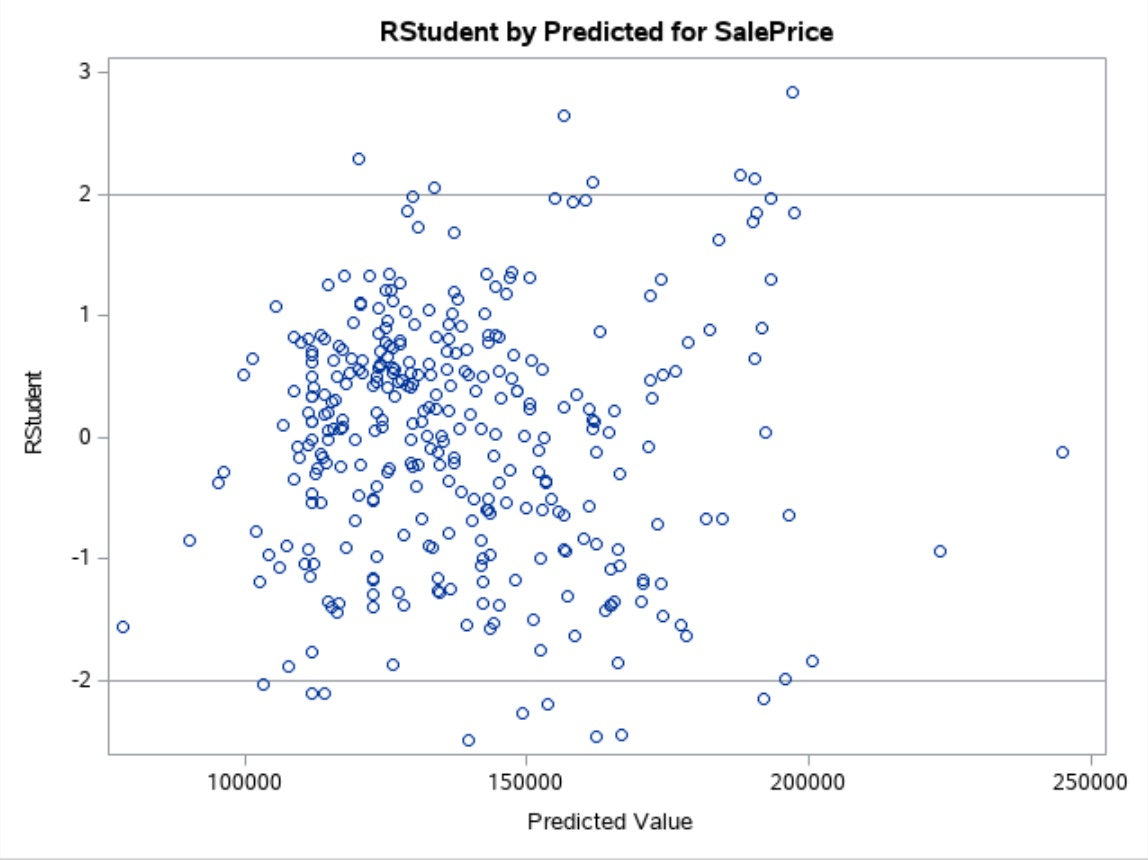
\includegraphics[width=0.23\textwidth]{../graphics/A1StudentResiduals2}}\\
		\hline
	\end{tabular}		
	\caption{Residual Plots.}
	\label{fig:A1RP}
\end{figure}


\subsubsection{Assumptions}
\paragraph{Linearity} The linearity assumption is met by the reviewing the scatter plots associated with data. Fig ~\ref{fig:A1LR} shows a plot of SalePrice vs. GrLivArea and by removing the outliers the linearity assumption is reasonably met. 
\paragraph{Constant Variance} The residual plot, Fig ~\ref{fig:A1RP} resembles somewhat of a random scatter of points around the 0 line, although there is a slight suspicion of non-constant variance judging from the dense cloud around the predicted value of \$130,000. Also shown is the Studentized Residual Plot which is very similar to the residual plot, although this plot identifies potential outlying observations.
\paragraph{Normality} Based upon the histograms and q-q plots in Fig ~\ref{fig:A1QQ} there is no evidence to suggest that normality of the data. Additionally the random scatter associated with the residual plots in Fig ~\ref{fig:A1RP} also support the normality assumption.
\paragraph{Independence} The independence assumption can be assumed to be maintained since these are all unique sales in a free housing market. 
\subsubsection{Outliers and Influential Points}
\begin{figure}[h] % [h] forces the figure to be output where it is defined in the code (it suppresses floating)
	\centering
	\begin{tabular}{p{0.23\textwidth} p{0.23\textwidth}p{0.23\textwidth}p{0.23\textwidth}}
\hline	
	\multicolumn{2}{|c|}{Original} &  \multicolumn{2}{|c|}{After Removal of Outliers} \\
		\multicolumn{1}{|c}{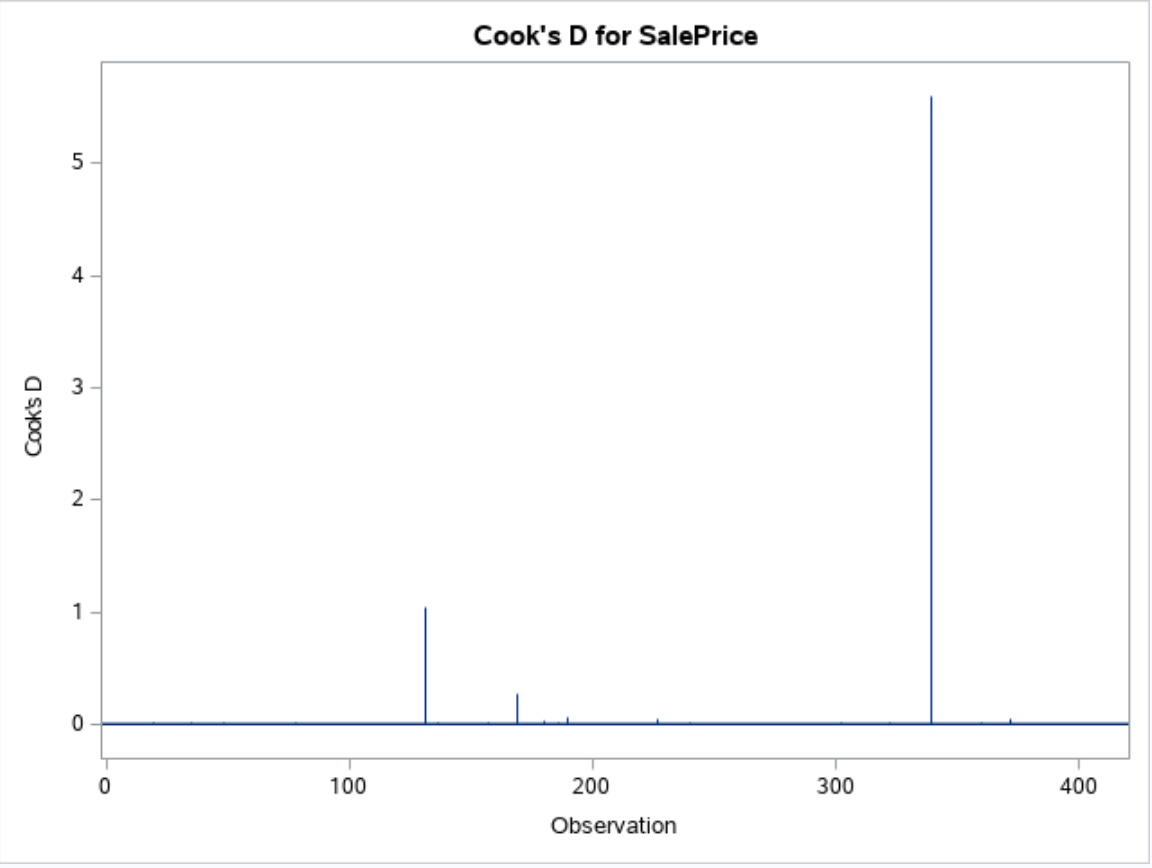
\includegraphics[width=0.23\textwidth]{../graphics/A1Cooks1}} &
		\multicolumn{1}{c|}{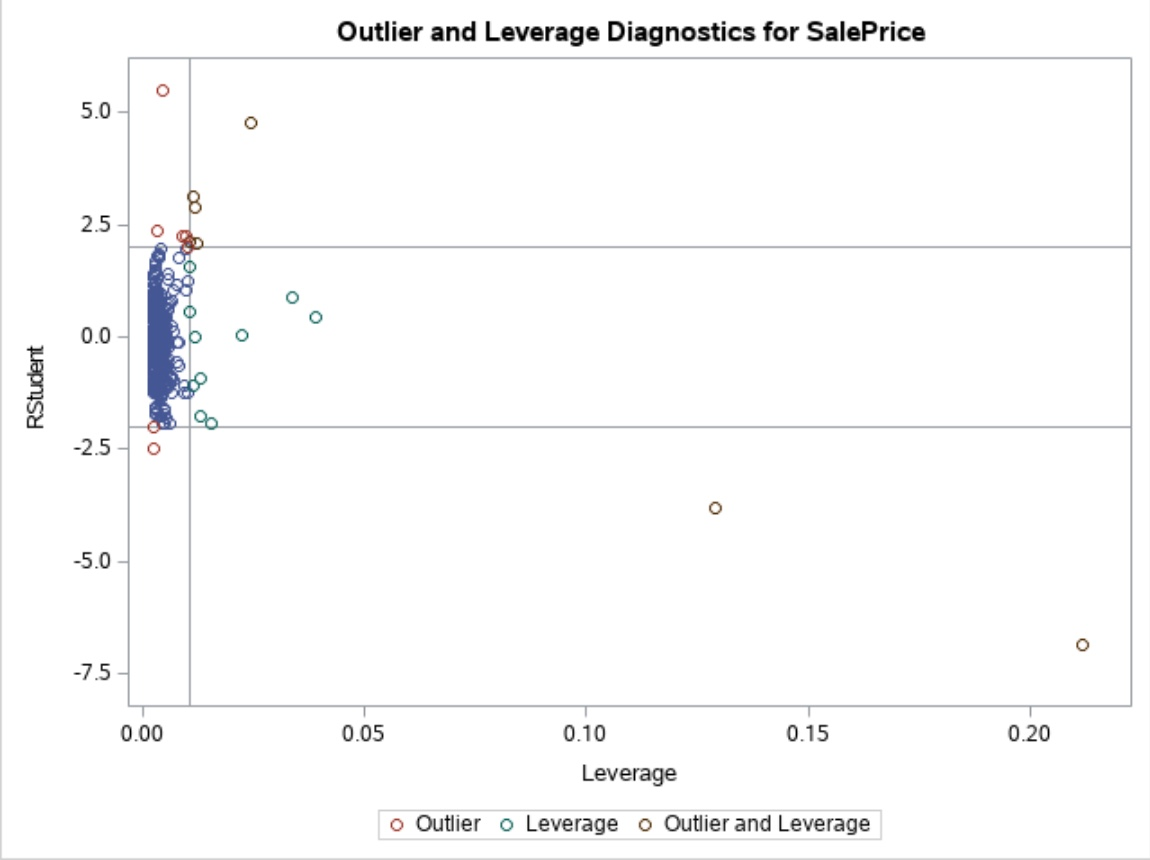
\includegraphics[width=0.23\textwidth]{../graphics/A1Lev1}} &
		\multicolumn{1}{|c}{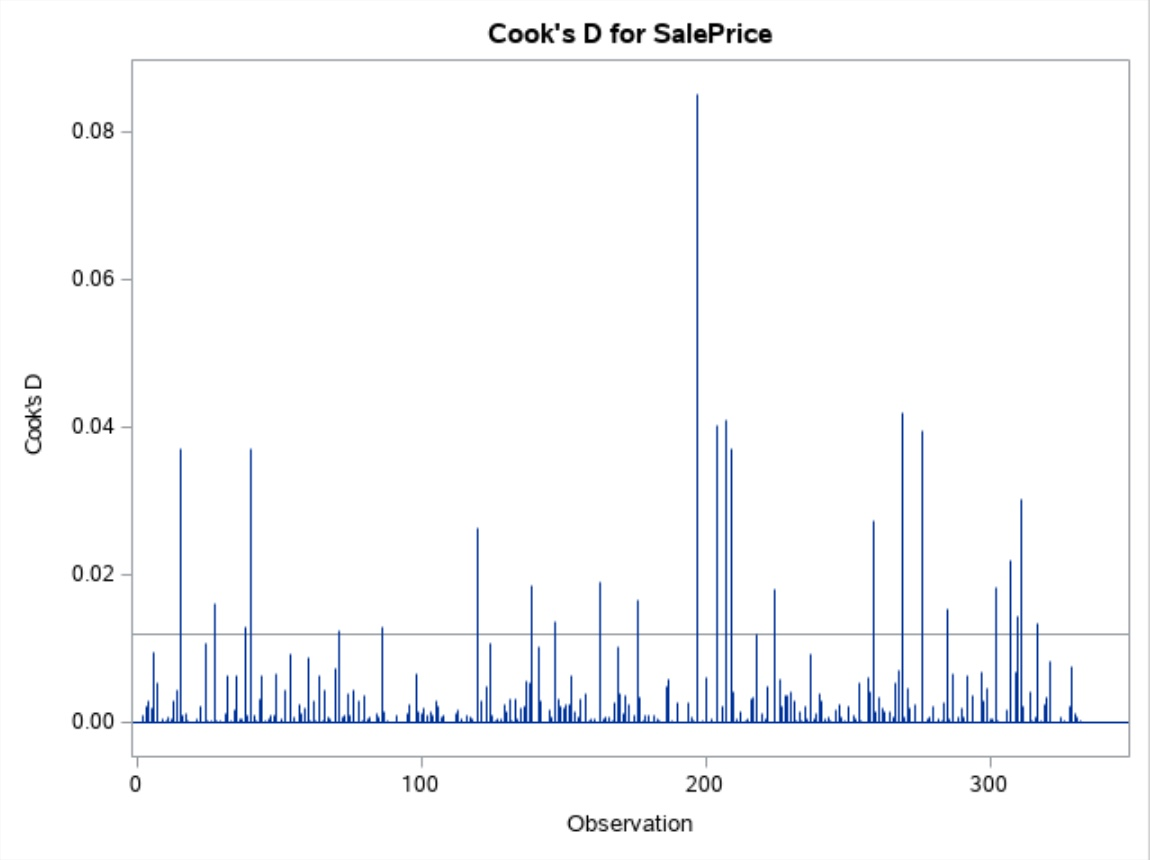
\includegraphics[width=0.23\textwidth]{../graphics/A1Cooks2}} &
		\multicolumn{1}{c|}{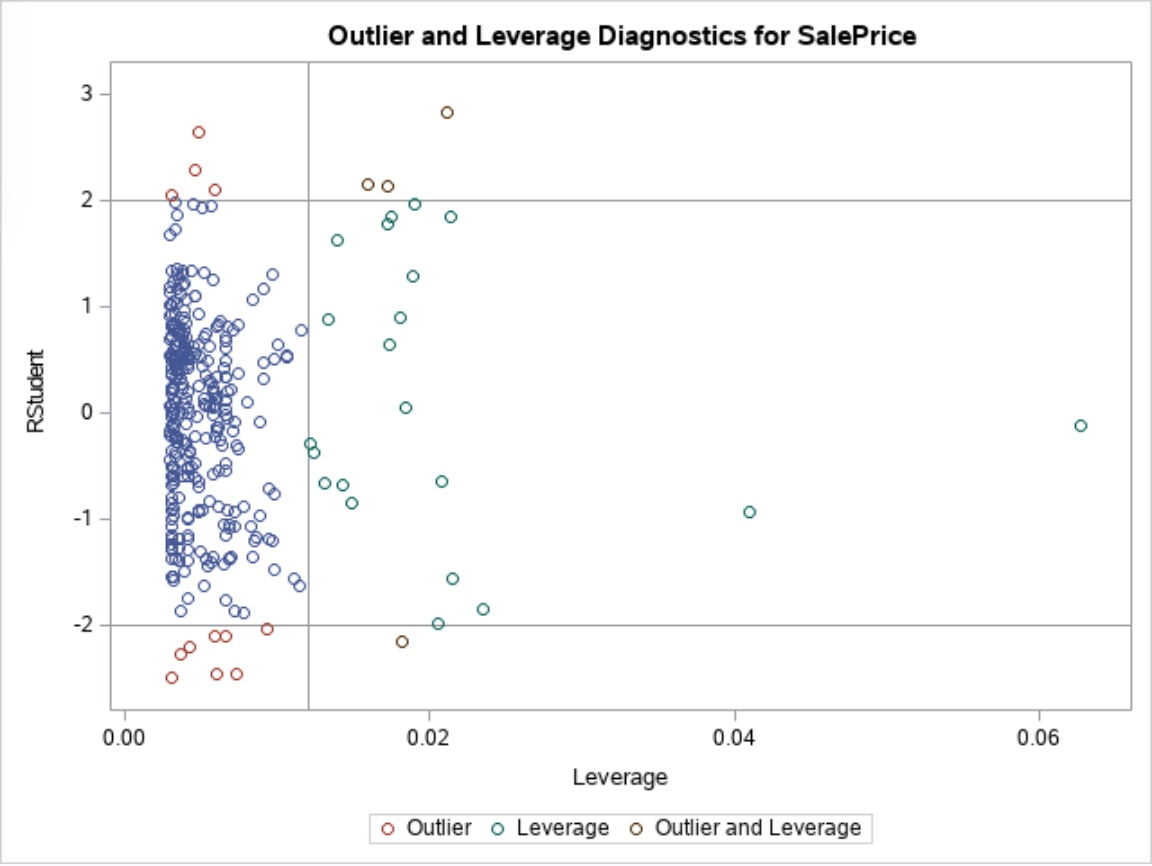
\includegraphics[width=0.23\textwidth]{../graphics/A1Lev2}}\\
		\hline
	\end{tabular}		
	\caption{Influential Point Plots.}
	\label{fig:A1IP}
\end{figure}
\paragraph{outliers / influential observations} There are distinct outliers that can be seen both in the Cook's D and Outlier and Leverage Diagnostics seen in Fig ~\ref{fig:A1IP}. By removing the observations that resulted from non-normal sales conditions such as foreclosures and sale prices that were significantly outside the population, the Cook's D and Outlier and Leverage Diagnostics significantly improved. We are confident that the removal of these observations was appropriate since they do not represent the population as a whole. Additionally we are confident that the remaining data does not contain significant outliers or leverage points that need to be addressed further.
\paragraph{}The model is a reasonable fit without transformations.  The removal of observations not reflective of the population, such as non-normal sale conditions and home sales greater than \$300,000, seems appropriate and enables the required model assumptions to be met.

\subsubsection{Effect by Neighborhood}
\begin{figure}[h] % [h] forces the figure to be output where it is defined in the code (it suppresses floating)
	\centering
	\begin{tabular}{p{0.48\textwidth} p{0.48\textwidth}}
\hline	
	\multicolumn{1}{|c|}{Original} &  \multicolumn{1}{|c|}{After Removal of Outliers} \\
		\multicolumn{1}{|c|}{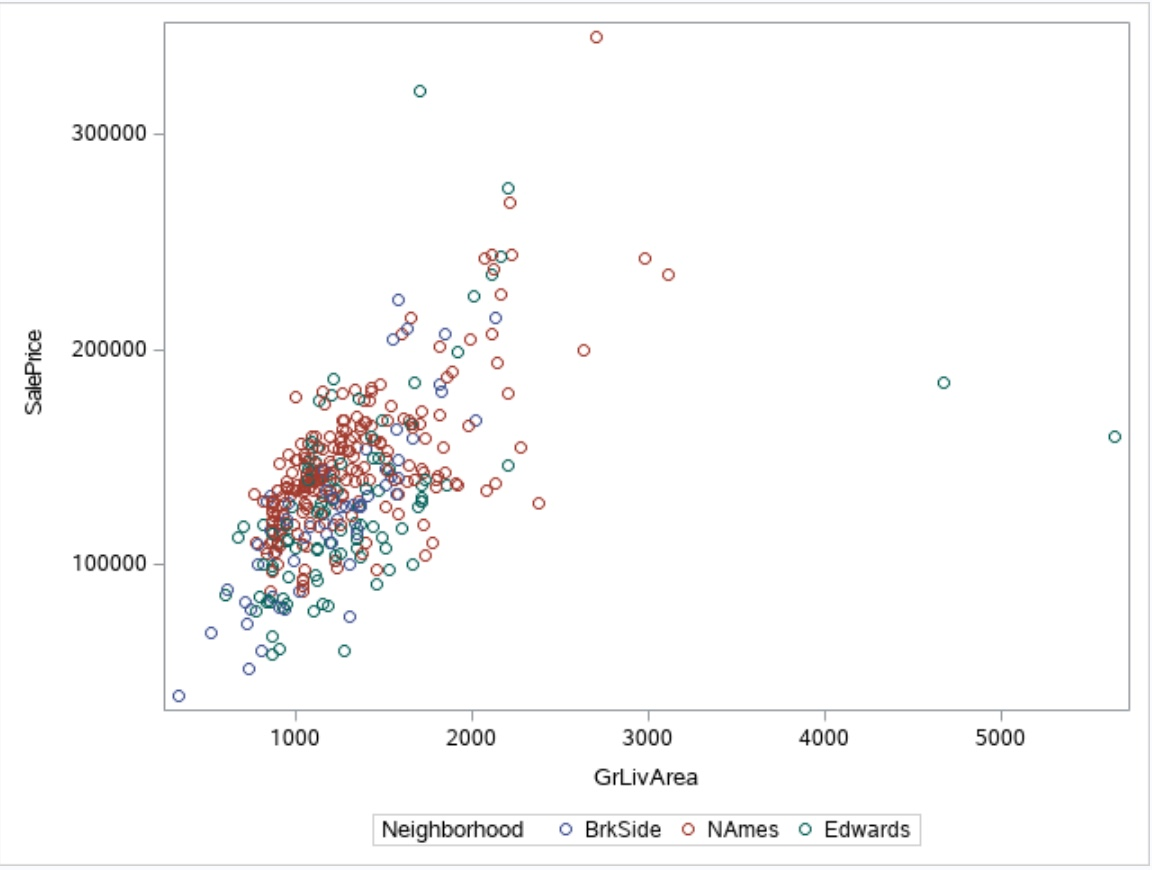
\includegraphics[width=0.48\textwidth]{../graphics/A1NHscat1}} &
		\multicolumn{1}{|c|}{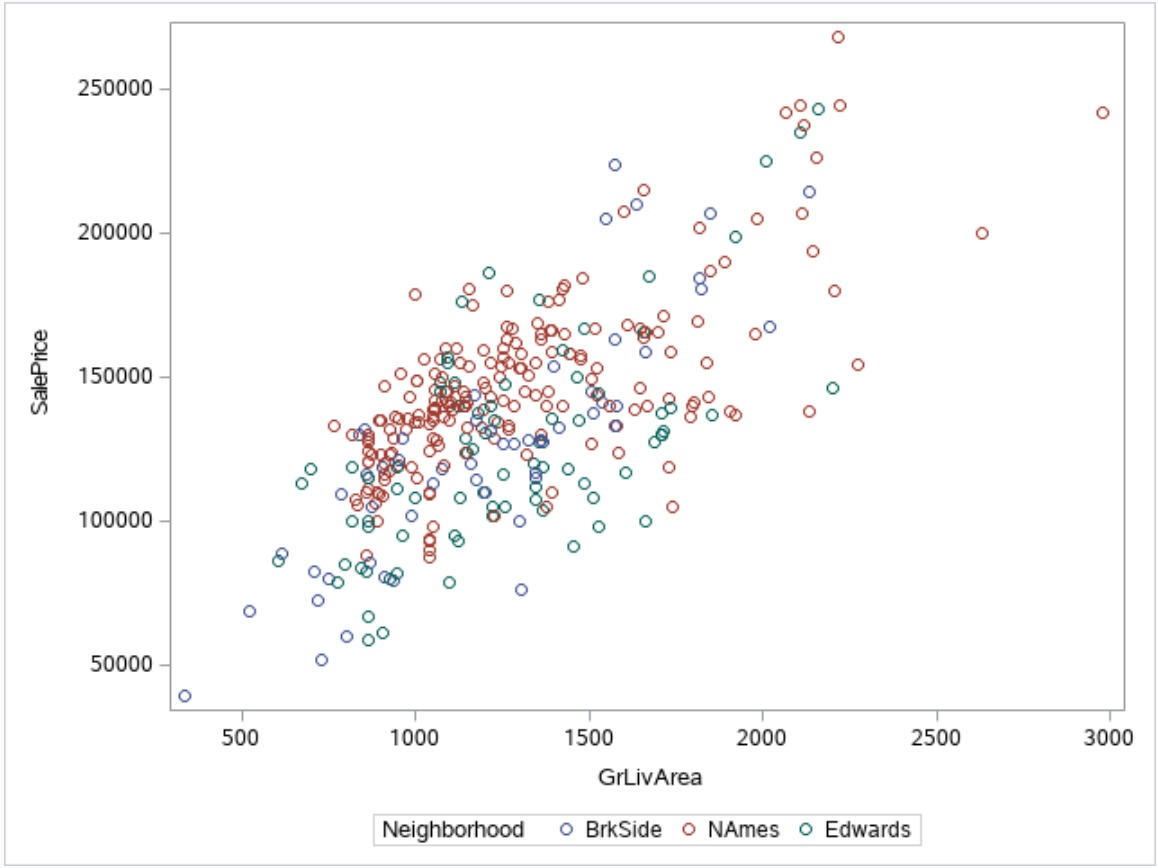
\includegraphics[width=0.48\textwidth]{../graphics/A1NHscat2}}\\
		\hline
	\end{tabular}		
	\caption{Scatterplot of Sale Prices vs Living Area by Neighborhood.}
	\label{fig:NBscat}
\end{figure}
\paragraph{Model} A model was developed to individually look at the neighborhoods of interest to determine if the sale price is impacted by neighborhood. Fig ~\ref{fig:NBscat} shows the sales price vs living area by neighborhood. The model shows (Table~\ref{tab:SMM}) that the intercept and slope for Brookside and Edwards do differ from North Ames with statistical significance (p-values: $<.0001$ and $.0077$). As such we have determined to choose this model which allows for different intercept and slopes based upon the neighborhood. The resultant model can be seen in Fig ~\ref{fig:NBLRM}.
\begin{table}[h] % [h] forces the table to be output where it is defined in the code (it suppresses floating)
	\centering % Centre the table
	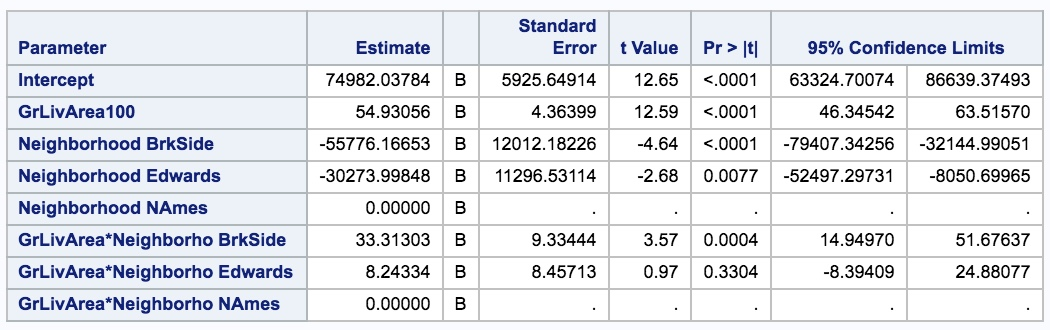
\includegraphics[scale=.3]{../graphics/A1NHcomp}
	\caption{Results of Neighborhood Impact on Sales Price}
	\label{tab:SMM}
\end{table}

\begin{figure}[h] % [h] forces the figure to be output where it is defined in the code (it suppresses floating)
	\centering
	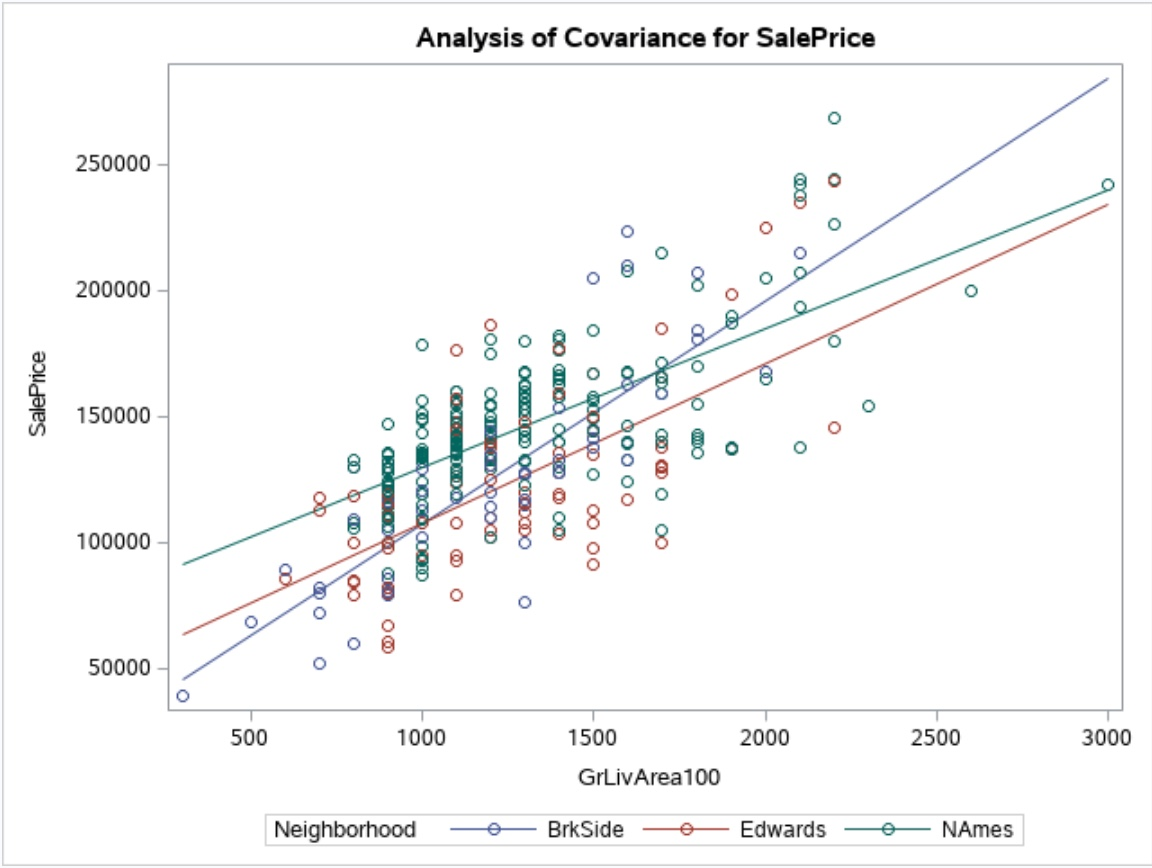
\includegraphics[scale=.2]{../graphics/A1NBMLR}
	\caption{Linear Regression Model by Neighborhood.}
	\label{fig:NBLRM}
\end{figure}
%------------------------------------------------

\subsection{Model Metrics}
Model metrics can be seen in Table ~\ref{tab:A1Results}.
\begin{table}[h] % [h] forces the table to be output where it is defined in the code (it suppresses floating)
	\centering % Centre the table
	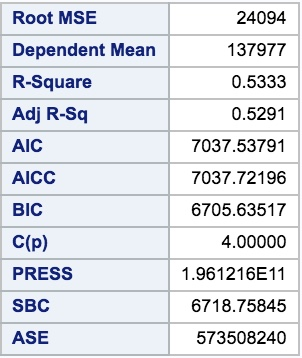
\includegraphics[scale=.4]{../graphics/A1NBMLRResults}
	\caption{Results of Neighborhood Impact on Sales Price}
	\label{tab:A1Results}
\end{table}
\subsubsection{Adj R\textsuperscript{2}} 
\paragraph{Adjusted $R^2$} obtained for this model is 0.53.
\subsubsection{Internal Press} 
\paragraph{Press} obtained by this model is $1.96E11$.
%------------------------------------------------

\subsection{Parameters}
\subsubsection{Estimates}
\paragraph{} The parameter estimates can be seen in Table ~\ref{tab:SMM}. With these estimates a separate equation can be written for each neighborhood to predict sale price based on living area.
\begin{eqnarray*}
SalePrice &=& 74982 + 54.93(GrLivArea) - 55776(BrkSide) - 30274(Edwards) + \\
& & 33.31(GrLivArea)(BrkSide) + 8.24(GrLivArea)(Edwards)\\
\end{eqnarray*}
\paragraph{North Ames}
\begin{eqnarray*}
SalePrice &=& 74982 + 54.93(GrLivArea)\\
\end{eqnarray*}
\paragraph{Edwards}
\begin{eqnarray*}
SalePrice &=& 74982 + 54.93(GrLivArea) - 30274 + 8.24(GrLivArea)\\
&=& 44708 + 63.17(GrLivArea)\\
\end{eqnarray*}
\paragraph{Brookside}
\begin{eqnarray*}
SalePrice &=& 74982 + 54.93(GrLivArea) - 55776 + 33.31(GrLivArea)\\
&=& 19206 + 88.24(GrLivArea)\\
\end{eqnarray*}
\subsubsection{Interpretation}
\paragraph{$\beta_0$}The intercept in this model provides an estimate (74982) of the sale price of a home in North Ames (reference neighborhood) with a living area of zero. Of course, this is extrapolation and does not have a clear, practical meaning.
\paragraph{$\beta_1$}For each 100 square foot increase in the living area of a home in North Ames, the estimated sale price increases \$54.93.
\paragraph{$\beta_2$}This is the adjustment of the intercept for a home in Brookside with respect to a home in North Ames. For a living area of zero, the home in Brookside has an estimated sale price of \$55,776 less than a home in North Ames.
\paragraph{$\beta_3$}This is the adjustment of the intercept for a home in Edwards with respect to a home in North Ames. For a living area of zero, the home in Edwards has an estimated sale price of \$30,274 less than a home in North Ames.
\paragraph{$\beta_4$}For each 100 square foot increase in the living area of a home in Brookside, the estimated sale price increases \$33 from the change with the home in North Ames.
\paragraph{$\beta_5$}For each 100 square foot increase in the living area of a home in Edwards, the estimated sale price increases \$8 from the change with the home in North Ames.
\subsubsection{Confidence Intervals}
The confidence intervals for the estimates can be seen in Table ~\ref{tab:SMM}. 
%------------------------------------------------

\subsection{Conclusion}
\paragraph{} The square feet of above ground living area is a statistically significant feature to use to predict the sale price of homes in the North Ames, Edwards, and Brookside neighborhoods of Ames, Iowa. The existing sale prices of homes that have sold in these neighborhoods that are under \$300,000 and underwent a normal sales condition meet all the assumptions required to generate an appropriate linear regression model. We also examined the differences in predicted prices in these three neighborhoods and determined that the sale prices of homes in each of these neighborhoods do differ from each other. Homes in North Ames under 1600 square feet are predicted to sell for the highest price as compared to the other two neighborhoods. The price per square foot in Brookside increases at the highest rate of the three neighborhoods. Homes greater than approximately 1000 square feet in Brookside are predicted to sell for higher prices than comparable homes in Edwards. Homes greater than approximately 1600 square feet in Brookside are predicted to sell for higher prices than comparable homes in North Ames. Homes in the Edwards neighborhood are predicted to sell for the lowest price of all three neighbor hoods with the exception of homes that are smaller than 1000 square feet.
%------------------------------------------------

\section{Analysis Question 2}
%------------------------------------------------

\subsection{Restatement of Problem}
\paragraph{} Build the most predictive model for sales prices of homes in all of Ames Iowa.  This includes all neighborhoods. Your group is limited to only the techniques we have learned in 6371 (no random forests or other methods we have not yet covered).  Specifically, you should produce 4 models: one from forward selection, one from backwards elimination, one from stepwise selection, and one that you build custom.  The custom model could be one of the three preceding models or one that you build by adding or subtracting variables at your will.  Generate an adjusted R2, CV Press and Kaggle Score for each of these models and clearly describe which model you feel is the best in terms of being able to predict future sale prices of homes in Ames, Iowa. 
%------------------------------------------------

\subsection{Model Selection}
\subsubsection{Stepwise}
\subsubsection{Forward}
\subsubsection{Backward}
\subsubsection{Custom}
%------------------------------------------------

\subsection{Checking Assumptions}
\subsubsection{Residual Plots}
\subsubsection{Influential point analysis (Cook’s D and Leverage)}
\subsubsection{Make sure to address each assumption}
%------------------------------------------------

\subsection{Comparing Competing Models}
\begin{table}[h] % [h] forces the table to be output where it is defined in the code (it suppresses floating)
	\centering % Centre the table
\begin{tabular}{|l|l|l|l|}
\hline
\textbf{Predictive Models} & \textbf{Adjusted R\textsuperscript{2}} & \textbf{CV Press} & \textbf{Kaggle Score}\\
\hline
Forward & XX & XX & XX\\
\hline
Backward & XX & XX & XX\\
\hline
Stepwise & XX & XX & XX\\
\hline
CUSTOM & XX & XX & XX\\
\hline
\end{tabular}
\caption{Analysis Results}
\end{table}
\subsubsection{Adj R\textsuperscript{2}}
\subsubsection{Internal CV Press}
\subsubsection{Kaggle Score}
%------------------------------------------------

\subsection{Conclusion}

%------------------------------------------------

%% ------------------------------------------
%% this restarts the section numbering and
%% changes chapter numbering to letters starting
%% with A
%% ------------------------------------------
\appendix{} 

\pagebreak
\section{Source Code for Analysis 1}
\label{sec:Analysis1}
\lstinputlisting[
	caption=Analysis 1 SAS Code., % Caption above the listing
	label=lst:Analysis1Source, % Label for referencing this listing
	language=SAS, % Use SAS functions/syntax highlighting
	frame=single, % Frame around the code listing
	showstringspaces=false, % Don't put marks in string spaces
	numbers=left, % Line numbers on left
	numberstyle=\tiny, % Line numbers styling
	]{../code/Analysis1.sas}

%------------------------------------------------

\pagebreak

\section{Source Code for Analysis 2}
\label{sec:Analysis2}

\subsection{Forward Selection}
\lstinputlisting[
	caption=Forward Selection SAS Code., % Caption above the listing
	label=lst:Forward, % Label for referencing this listing
	language=SAS, % Use SAS functions/syntax highlighting
	frame=single, % Frame around the code listing
	showstringspaces=false, % Don't put marks in string spaces
	numbers=left, % Line numbers on left
	numberstyle=\tiny, % Line numbers styling
	]{../code/Forward.sas}

\subsection{Backward Selection}
\lstinputlisting[
	caption=Backward Selection SAS Code., % Caption above the listing
	label=lst:Backward, % Label for referencing this listing
	language=SAS, % Use SAS functions/syntax highlighting
	frame=single, % Frame around the code listing
	showstringspaces=false, % Don't put marks in string spaces
	numbers=left, % Line numbers on left
	numberstyle=\tiny, % Line numbers styling
	]{../code/Backward.sas}

\subsection{Stepwise Selection}
\lstinputlisting[
	caption=Stepwise Selection SAS Code., % Caption above the listing
	label=lst:Stepwise, % Label for referencing this listing
	language=SAS, % Use SAS functions/syntax highlighting
	frame=single, % Frame around the code listing
	showstringspaces=false, % Don't put marks in string spaces
	numbers=left, % Line numbers on left
	numberstyle=\tiny, % Line numbers styling
	]{../code/Stepwise.sas}	
%------------------------------------------------
\pagebreak
\section{High Level Summary of Data}
\begin{table}[h] % [h] forces the table to be output where it is defined in the code (it suppresses floating)
	\centering % Centre the table
	\begin{tabular}{|l l l l l|}
		\hline
		\multicolumn{3}{|l|}{Attribute} & \multicolumn{1}{|l|}{} & \multicolumn{1}{|l|}{}\\
		\multicolumn{3}{|l|}{Type} & \multicolumn{1}{|l|}{Description} & \multicolumn{1}{|l|}{Features}\\
		\hline
		& & \multicolumn{1}{|l|}{} & \multicolumn{1}{|l|}{Only provide}& \multicolumn{1}{|l|}{MSSubClass, MSZoning, Street, Alley, LotShape,} \\
		 &  & \multicolumn{1}{|l|}{} & \multicolumn{1}{|l|}{enough information}& \multicolumn{1}{|l|}{LandContour, Utilities, LotConfig, LandSlope,}\\
		& & \multicolumn{1}{|l|}{Nominal} & \multicolumn{1}{|l|}{to distinguish one}& \multicolumn{1}{|l|}{Neighborhood, Condition1, Condition2, BldgType,} \\
& & \multicolumn{1}{|l|}{} & \multicolumn{1}{|l|}{object from another}& \multicolumn{1}{|l|}{HouseStyle, RoofMatl, Exterior1st, Exterior2nd,} \\
		\multirow{2}{*}{\STAB{\rotatebox[origin=c]{90}{Categorical}}}		& \multirow{2}{*}{\STAB{\rotatebox[origin=c]				{90}{(Qualitative)}}}& \multicolumn{1}{|l|}{} & \multicolumn{1}{|l|}{}& \multicolumn{1}{|l|}{MasVnrType, Foundation, BsmtExposure, Heating} \\
				& & \multicolumn{1}{|l|}{} & \multicolumn{1}{|l|}{}& \multicolumn{1}{|l|}{CentralAir, Electrical, GarageType, GarageFinish} \\
				& & \multicolumn{1}{|l|}{} & \multicolumn{1}{|l|}{}& \multicolumn{1}{|l|}{PavedDrive, MiscFeature, SaleType, SaleCondition} \\	
				& & \multicolumn{1}{|l|}{} & \multicolumn{1}{|l|}{}& \multicolumn{1}{|l|}{RoofStyle \textbf{(30 variables)}} \\
			\cline{3-5}
		& & \multicolumn{1}{|l|}{} & \multicolumn{1}{|l|}{Provide enough}& \multicolumn{1}{|l|}{OverallQual, OverallCond, ExterQual, ExterCond,} \\
		& & \multicolumn{1}{|l|}{Ordinal} & \multicolumn{1}{|l|}{information to}& \multicolumn{1}{|l|}{BsmtQual, BsmtCond, BsmtFinType1,} \\
				& & \multicolumn{1}{|l|}{} & \multicolumn{1}{|l|}{order objects}& \multicolumn{1}{|l|}{BsmtFinType2, HeatingQC, KitchenQual, Functional,} \\
				& & \multicolumn{1}{|l|}{} & \multicolumn{1}{|l|}{}& \multicolumn{1}{|l|}{FireplaceQu, GarageQual, GarageCond, PoolQC,} \\					& & \multicolumn{1}{|l|}{} & \multicolumn{1}{|l|}{}& \multicolumn{1}{|l|}{Fence \textbf{(16 variables)}} \\				
\hline
		& & \multicolumn{1}{|l|}{} & \multicolumn{1}{|l|}{Interval attributes}& \multicolumn{1}{|l|}{YearBuilt, YearRemodAdd, GarageYrBlt, MoSold,} \\
		 &  & \multicolumn{1}{|l|}{Interval} & \multicolumn{1}{|l|}{difference between}& \multicolumn{1}{|l|}{YrSold \textbf{(5 variables)}}\\
		& & \multicolumn{1}{|l|}{} & \multicolumn{1}{|l|}{values are}& \multicolumn{1}{|l|}{} \\
	& \multirow{2}{*}{\STAB{\rotatebox[origin=c]				{90}{(Quantitative)}}}& \multicolumn{1}{|l|}{} & \multicolumn{1}{|l|}{meaningful}& \multicolumn{1}{|l|}{} \\
		\cline{3-5}
\multirow{2}{*}{\STAB{\rotatebox[origin=c]{90}{Numeric}}}			& & \multicolumn{1}{|l|}{} & \multicolumn{1}{|l|}{Differences and}& \multicolumn{1}{|l|}{LotFrontage, LotArea, BsmtFinSF1, BsmtFinSF2,} \\
		& & \multicolumn{1}{|l|}{Ratio} & \multicolumn{1}{|l|}{ratios are}& \multicolumn{1}{|l|}{BsmtUnfSF, TotalBsmtSF, 1stFlrSF, 2ndFlrSF,} \\
				& & \multicolumn{1}{|l|}{} & \multicolumn{1}{|l|}{meaningful}& \multicolumn{1}{|l|}{LowQualFinSF, GrLivArea, BsmtFullBath,} \\
								& & \multicolumn{1}{|l|}{} & \multicolumn{1}{|l|}{}& \multicolumn{1}{|l|}{MasVnrArea, BsmtHalfBath, FullBath, HalfBath,} \\
& & \multicolumn{1}{|l|}{} & \multicolumn{1}{|l|}{}& \multicolumn{1}{|l|}{Bedroom, Kitchen, TotRmsAbvGrd, Fireplaces,} \\
& & \multicolumn{1}{|l|}{} & \multicolumn{1}{|l|}{}& \multicolumn{1}{|l|}{GarageCars, GarageArea, WoodDeckSF, OpenPorchSF,} \\
& & \multicolumn{1}{|l|}{} & \multicolumn{1}{|l|}{}& \multicolumn{1}{|l|}{EnclosedPorch, 3SsnPorch, ScreenPorch, PoolArea,} \\
& & \multicolumn{1}{|l|}{} & \multicolumn{1}{|l|}{}& \multicolumn{1}{|l|}{MiscVal \textbf{(28 variables)}} \\
\hline

	\end{tabular}
	\caption{Summary of Dataset}
	\label{tab:Data}
\end{table}

\pagebreak
\section{Detailed Data Description}
\label{sec:DataDescription}
\begin{center}
\begin{tabular}{c c c c c c}
\hline
\multicolumn{6}{|c|}{Classification Variables}\\
\hline
\multicolumn{2}{|c}{MSSubClass} & \multicolumn{4}{l|}{Identifies the type of dwelling involved in the sale}\\ \multicolumn{2}{|c}{} & \multicolumn{1}{c}{20} & \multicolumn{3}{l|}{1-STORY 1946 \& NEWER ALL STYLES}\\
\multicolumn{2}{|c}{} & \multicolumn{1}{c}{30} & \multicolumn{3}{l|}{1-STORY 1945 \& OLDER}\\
\multicolumn{2}{|c}{} & \multicolumn{1}{c}{40} & \multicolumn{3}{l|}{1-STORY W/FINISHED ATTIC ALL AGES}\\
\multicolumn{2}{|c}{} & \multicolumn{1}{c}{45} & \multicolumn{3}{l|}{1-1/2 STORY - UNFINISHED ALL AGES}\\
\multicolumn{2}{|c}{} & \multicolumn{1}{c}{50} & \multicolumn{3}{l|}{1-1/2 STORY FINISHED ALL AGES}\\
\multicolumn{2}{|c}{} & \multicolumn{1}{c}{60} & \multicolumn{3}{l|}{2-STORY 1946 \& NEWER}\\
\multicolumn{2}{|c}{} & \multicolumn{1}{c}{70} & \multicolumn{3}{l|}{2-STORY 1945 \& OLDER}\\
\multicolumn{2}{|c}{} & \multicolumn{1}{c}{75} & \multicolumn{3}{l|}{2-1/2 STORY ALL AGES}\\
\multicolumn{2}{|c}{} & \multicolumn{1}{c}{80} & \multicolumn{3}{l|}{SPLIT OR MULTI-LEVEL}\\
\multicolumn{2}{|c}{} & \multicolumn{1}{c}{85} & \multicolumn{3}{l|}{SPLIT FOYER}\\
\multicolumn{2}{|c}{} & \multicolumn{1}{c}{90} & \multicolumn{3}{l|}{DUPLEX - ALL STYLES AND AGES}\\
\multicolumn{2}{|c}{} & \multicolumn{1}{c}{120} & \multicolumn{3}{l|}{1-STORY PUD (Planned Unit Development) - 1946 \& NEWER}\\
\multicolumn{2}{|c}{} & \multicolumn{1}{c}{150} & \multicolumn{3}{l|}{1-1/2 STORY PUD - ALL AGES}\\
\multicolumn{2}{|c}{} & \multicolumn{1}{c}{160} & \multicolumn{3}{l|}{2-STORY PUD - 1946 \& NEWER}\\
\multicolumn{2}{|c}{} & \multicolumn{1}{c}{180} & \multicolumn{3}{l|}{PUD - MULTILEVEL - INCL SPLIT LEV/FOYER}\\
\multicolumn{2}{|c}{} & \multicolumn{1}{c}{190} & \multicolumn{3}{l|}{2 FAMILY CONVERSION - ALL STYLES AND AGES}\\
\hline
\end{tabular}
\end{center}
\end{document}
MSZoning: Identifies the general zoning classification of the sale.
		
       A	Agriculture
       C	Commercial
       FV	Floating Village Residential
       I	Industrial
       RH	Residential High Density
       RL	Residential Low Density
       RP	Residential Low Density Park 
       RM	Residential Medium Density
	
LotFrontage: Linear feet of street connected to property

LotArea: Lot size in square feet

Street: Type of road access to property

       Grvl	Gravel	
       Pave	Paved
       	
Alley: Type of alley access to property

       Grvl	Gravel
       Pave	Paved
       NA 	No alley access
		
LotShape: General shape of property

       Reg	Regular	
       IR1	Slightly irregular
       IR2	Moderately Irregular
       IR3	Irregular
       
LandContour: Flatness of the property

       Lvl	Near Flat/Level	
       Bnk	Banked - Quick and significant rise from street grade to building
       HLS	Hillside - Significant slope from side to side
       Low	Depression
		
Utilities: Type of utilities available
		
       AllPub	All public Utilities (E,G,W,& S)	
       NoSewr	Electricity, Gas, and Water (Septic Tank)
       NoSeWa	Electricity and Gas Only
       ELO	Electricity only	
	
LotConfig: Lot configuration

       Inside	Inside lot
       Corner	Corner lot
       CulDSac	Cul-de-sac
       FR2	Frontage on 2 sides of property
       FR3	Frontage on 3 sides of property
	
LandSlope: Slope of property
		
       Gtl	Gentle slope
       Mod	Moderate Slope	
       Sev	Severe Slope
	
Neighborhood: Physical locations within Ames city limits

       Blmngtn	Bloomington Heights
       Blueste	Bluestem
       BrDale	Briardale
       BrkSide	Brookside
       ClearCr	Clear Creek
       CollgCr	College Creek
       Crawfor	Crawford
       Edwards	Edwards
       Gilbert	Gilbert
       IDOTRR	Iowa DOT and Rail Road
       MeadowV	Meadow Village
       Mitchel	Mitchell
       Names	North Ames
       NoRidge	Northridge
       NPkVill	Northpark Villa
       NridgHt	Northridge Heights
       NWAmes	Northwest Ames
       OldTown	Old Town
       SWISU	South & West of Iowa State University
       Sawyer	Sawyer
       SawyerW	Sawyer West
       Somerst	Somerset
       StoneBr	Stone Brook
       Timber	Timberland
       Veenker	Veenker
			
Condition1: Proximity to various conditions
	
       Artery	Adjacent to arterial street
       Feedr	Adjacent to feeder street	
       Norm	Normal	
       RRNn	Within 200' of North-South Railroad
       RRAn	Adjacent to North-South Railroad
       PosN	Near positive off-site feature--park, greenbelt, etc.
       PosA	Adjacent to postive off-site feature
       RRNe	Within 200' of East-West Railroad
       RRAe	Adjacent to East-West Railroad
	
Condition2: Proximity to various conditions (if more than one is present)
		
       Artery	Adjacent to arterial street
       Feedr	Adjacent to feeder street	
       Norm	Normal	
       RRNn	Within 200' of North-South Railroad
       RRAn	Adjacent to North-South Railroad
       PosN	Near positive off-site feature--park, greenbelt, etc.
       PosA	Adjacent to postive off-site feature
       RRNe	Within 200' of East-West Railroad
       RRAe	Adjacent to East-West Railroad
	
BldgType: Type of dwelling
		
       1Fam	Single-family Detached	
       2FmCon	Two-family Conversion; originally built as one-family dwelling
       Duplx	Duplex
       TwnhsE	Townhouse End Unit
       TwnhsI	Townhouse Inside Unit
	
HouseStyle: Style of dwelling
	
       1Story	One story
       1.5Fin	One and one-half story: 2nd level finished
       1.5Unf	One and one-half story: 2nd level unfinished
       2Story	Two story
       2.5Fin	Two and one-half story: 2nd level finished
       2.5Unf	Two and one-half story: 2nd level unfinished
       SFoyer	Split Foyer
       SLvl	Split Level
	
OverallQual: Rates the overall material and finish of the house

       10	Very Excellent
       9	Excellent
       8	Very Good
       7	Good
       6	Above Average
       5	Average
       4	Below Average
       3	Fair
       2	Poor
       1	Very Poor
	
OverallCond: Rates the overall condition of the house

       10	Very Excellent
       9	Excellent
       8	Very Good
       7	Good
       6	Above Average	
       5	Average
       4	Below Average	
       3	Fair
       2	Poor
       1	Very Poor
		
YearBuilt: Original construction date

YearRemodAdd: Remodel date (same as construction date if no remodeling or additions)

RoofStyle: Type of roof

       Flat	Flat
       Gable	Gable
       Gambrel	Gabrel (Barn)
       Hip	Hip
       Mansard	Mansard
       Shed	Shed
		
RoofMatl: Roof material

       ClyTile	Clay or Tile
       CompShg	Standard (Composite) Shingle
       Membran	Membrane
       Metal	Metal
       Roll	Roll
       Tar&Grv	Gravel & Tar
       WdShake	Wood Shakes
       WdShngl	Wood Shingles
		
Exterior1st: Exterior covering on house

       AsbShng	Asbestos Shingles
       AsphShn	Asphalt Shingles
       BrkComm	Brick Common
       BrkFace	Brick Face
       CBlock	Cinder Block
       CemntBd	Cement Board
       HdBoard	Hard Board
       ImStucc	Imitation Stucco
       MetalSd	Metal Siding
       Other	Other
       Plywood	Plywood
       PreCast	PreCast	
       Stone	Stone
       Stucco	Stucco
       VinylSd	Vinyl Siding
       Wd Sdng	Wood Siding
       WdShing	Wood Shingles
	
Exterior2nd: Exterior covering on house (if more than one material)

       AsbShng	Asbestos Shingles
       AsphShn	Asphalt Shingles
       BrkComm	Brick Common
       BrkFace	Brick Face
       CBlock	Cinder Block
       CemntBd	Cement Board
       HdBoard	Hard Board
       ImStucc	Imitation Stucco
       MetalSd	Metal Siding
       Other	Other
       Plywood	Plywood
       PreCast	PreCast
       Stone	Stone
       Stucco	Stucco
       VinylSd	Vinyl Siding
       Wd Sdng	Wood Siding
       WdShing	Wood Shingles
	
MasVnrType: Masonry veneer type

       BrkCmn	Brick Common
       BrkFace	Brick Face
       CBlock	Cinder Block
       None	None
       Stone	Stone
	
MasVnrArea: Masonry veneer area in square feet

ExterQual: Evaluates the quality of the material on the exterior 
		
       Ex	Excellent
       Gd	Good
       TA	Average/Typical
       Fa	Fair
       Po	Poor
		
ExterCond: Evaluates the present condition of the material on the exterior
		
       Ex	Excellent
       Gd	Good
       TA	Average/Typical
       Fa	Fair
       Po	Poor
		
Foundation: Type of foundation
		
       BrkTil	Brick & Tile
       CBlock	Cinder Block
       PConc	Poured Contrete	
       Slab	Slab
       Stone	Stone
       Wood	Wood
		
BsmtQual: Evaluates the height of the basement

       Ex	Excellent (100+ inches)	
       Gd	Good (90-99 inches)
       TA	Typical (80-89 inches)
       Fa	Fair (70-79 inches)
       Po	Poor (<70 inches
       NA	No Basement
		
BsmtCond: Evaluates the general condition of the basement

       Ex	Excellent
       Gd	Good
       TA	Typical - slight dampness allowed
       Fa	Fair - dampness or some cracking or settling
       Po	Poor - Severe cracking, settling, or wetness
       NA	No Basement
	
BsmtExposure: Refers to walkout or garden level walls

       Gd	Good Exposure
       Av	Average Exposure (split levels or foyers typically score average or above)	
       Mn	Mimimum Exposure
       No	No Exposure
       NA	No Basement
	
BsmtFinType1: Rating of basement finished area

       GLQ	Good Living Quarters
       ALQ	Average Living Quarters
       BLQ	Below Average Living Quarters	
       Rec	Average Rec Room
       LwQ	Low Quality
       Unf	Unfinshed
       NA	No Basement
		
BsmtFinSF1: Type 1 finished square feet

BsmtFinType2: Rating of basement finished area (if multiple types)

       GLQ	Good Living Quarters
       ALQ	Average Living Quarters
       BLQ	Below Average Living Quarters	
       Rec	Average Rec Room
       LwQ	Low Quality
       Unf	Unfinshed
       NA	No Basement

BsmtFinSF2: Type 2 finished square feet

BsmtUnfSF: Unfinished square feet of basement area

TotalBsmtSF: Total square feet of basement area

Heating: Type of heating
		
       Floor	Floor Furnace
       GasA	Gas forced warm air furnace
       GasW	Gas hot water or steam heat
       Grav	Gravity furnace	
       OthW	Hot water or steam heat other than gas
       Wall	Wall furnace
		
HeatingQC: Heating quality and condition

       Ex	Excellent
       Gd	Good
       TA	Average/Typical
       Fa	Fair
       Po	Poor
		
CentralAir: Central air conditioning

       N	No
       Y	Yes
		
Electrical: Electrical system

       SBrkr	Standard Circuit Breakers & Romex
       FuseA	Fuse Box over 60 AMP and all Romex wiring (Average)	
       FuseF	60 AMP Fuse Box and mostly Romex wiring (Fair)
       FuseP	60 AMP Fuse Box and mostly knob & tube wiring (poor)
       Mix	Mixed
		
1stFlrSF: First Floor square feet
 
2ndFlrSF: Second floor square feet

LowQualFinSF: Low quality finished square feet (all floors)

GrLivArea: Above grade (ground) living area square feet

BsmtFullBath: Basement full bathrooms

BsmtHalfBath: Basement half bathrooms

FullBath: Full bathrooms above grade

HalfBath: Half baths above grade

Bedroom: Bedrooms above grade (does NOT include basement bedrooms)

Kitchen: Kitchens above grade

KitchenQual: Kitchen quality

       Ex	Excellent
       Gd	Good
       TA	Typical/Average
       Fa	Fair
       Po	Poor
       	
TotRmsAbvGrd: Total rooms above grade (does not include bathrooms)

Functional: Home functionality (Assume typical unless deductions are warranted)

       Typ	Typical Functionality
       Min1	Minor Deductions 1
       Min2	Minor Deductions 2
       Mod	Moderate Deductions
       Maj1	Major Deductions 1
       Maj2	Major Deductions 2
       Sev	Severely Damaged
       Sal	Salvage only
		
Fireplaces: Number of fireplaces

FireplaceQu: Fireplace quality

       Ex	Excellent - Exceptional Masonry Fireplace
       Gd	Good - Masonry Fireplace in main level
       TA	Average - Prefabricated Fireplace in main living area or Masonry Fireplace in basement
       Fa	Fair - Prefabricated Fireplace in basement
       Po	Poor - Ben Franklin Stove
       NA	No Fireplace
		
GarageType: Garage location
		
       2Types	More than one type of garage
       Attchd	Attached to home
       Basment	Basement Garage
       BuiltIn	Built-In (Garage part of house - typically has room above garage)
       CarPort	Car Port
       Detchd	Detached from home
       NA	No Garage
		
GarageYrBlt: Year garage was built
		
GarageFinish: Interior finish of the garage

       Fin	Finished
       RFn	Rough Finished	
       Unf	Unfinished
       NA	No Garage
		
GarageCars: Size of garage in car capacity

GarageArea: Size of garage in square feet

GarageQual: Garage quality

       Ex	Excellent
       Gd	Good
       TA	Typical/Average
       Fa	Fair
       Po	Poor
       NA	No Garage
		
GarageCond: Garage condition

       Ex	Excellent
       Gd	Good
       TA	Typical/Average
       Fa	Fair
       Po	Poor
       NA	No Garage
		
PavedDrive: Paved driveway

       Y	Paved 
       P	Partial Pavement
       N	Dirt/Gravel
		
WoodDeckSF: Wood deck area in square feet

OpenPorchSF: Open porch area in square feet

EnclosedPorch: Enclosed porch area in square feet

3SsnPorch: Three season porch area in square feet

ScreenPorch: Screen porch area in square feet

PoolArea: Pool area in square feet

PoolQC: Pool quality
		
       Ex	Excellent
       Gd	Good
       TA	Average/Typical
       Fa	Fair
       NA	No Pool
		
Fence: Fence quality
		
       GdPrv	Good Privacy
       MnPrv	Minimum Privacy
       GdWo	Good Wood
       MnWw	Minimum Wood/Wire
       NA	No Fence
	
MiscFeature: Miscellaneous feature not covered in other categories
		
       Elev	Elevator
       Gar2	2nd Garage (if not described in garage section)
       Othr	Other
       Shed	Shed (over 100 SF)
       TenC	Tennis Court
       NA	None
		
MiscVal: $Value of miscellaneous feature

MoSold: Month Sold (MM)

YrSold: Year Sold (YYYY)

SaleType: Type of sale
		
       WD 	Warranty Deed - Conventional
       CWD	Warranty Deed - Cash
       VWD	Warranty Deed - VA Loan
       New	Home just constructed and sold
       COD	Court Officer Deed/Estate
       Con	Contract 15% Down payment regular terms
       ConLw	Contract Low Down payment and low interest
       ConLI	Contract Low Interest
       ConLD	Contract Low Down
       Oth	Other
		
SaleCondition: Condition of sale

       Normal	Normal Sale
       Abnorml	Abnormal Sale -  trade, foreclosure, short sale
       AdjLand	Adjoining Land Purchase
       Alloca	Allocation - two linked properties with separate deeds, typically condo with a garage unit	
       Family	Sale between family members
       Partial	Home was not completed when last assessed (associated with New Homes)


%----------------------------------------------------------------------------------------
%	COMMON TEMPLATE EXAMPLES
%----------------------------------------------------------------------------------------


%----------------------------------------------------------------------------------------
%	FIGURE EXAMPLE
%----------------------------------------------------------------------------------------

\begin{figure}[h] % [h] forces the figure to be output where it is defined in the code (it suppresses floating)
	\centering
	\includegraphics[width=0.5\columnwidth]{swallow.jpg} % Example image
	\caption{European swallow.}
\end{figure}

%------------------------------------------------


%----------------------------------------------------------------------------------------
%	TEXT EXAMPLE
%----------------------------------------------------------------------------------------

\section{Understanding Text}

\subsection{How much wood would a woodchuck chuck if a woodchuck could chuck wood?}

%------------------------------------------------

\subsubsection{Suppose ``chuck" implies throwing.}

According to the Associated Press (1988), a New York Fish and Wildlife technician named Richard Thomas calculated the volume of dirt in a typical 25--30 foot (7.6--9.1 m) long woodchuck burrow and had determined that if the woodchuck had moved an equivalent volume of wood, it could move ``about \textbf{700 pounds (320 kg)} on a good day, with the wind at his back".

%------------------------------------------------

\subsubsection{Suppose ``chuck" implies vomiting.}

A woodchuck can ingest 361.92 cm\textsuperscript{3} (22.09 cu in) of wood per day. Assuming immediate expulsion on ingestion with a 5\% retainment rate, a woodchuck could chuck \textbf{343.82 cm\textsuperscript{3}} of wood per day.

%------------------------------------------------

\paragraph{Bonus: suppose there is no woodchuck.}

Fusce varius orci ac magna dapibus porttitor. In tempor leo a neque bibendum sollicitudin. Nulla pretium fermentum nisi, eget sodales magna facilisis eu. Praesent aliquet nulla ut bibendum lacinia. Donec vel mauris vulputate, commodo ligula ut, egestas orci. Suspendisse commodo odio sed hendrerit lobortis. Donec finibus eros erat, vel ornare enim mattis et.

%----------------------------------------------------------------------------------------
%	EQUATION EXAMPLES
%----------------------------------------------------------------------------------------

\section{Interpreting Equations}

\subsection{Identify the author of Equation \ref{eq:bayes} below and briefly describe it in English.}

\begin{align} 
	\label{eq:bayes}
	\begin{split}
		P(A|B) = \frac{P(B|A)P(A)}{P(B)}
	\end{split}					
\end{align}

Lorem ipsum dolor sit amet, consectetur adipiscing elit. Praesent porttitor arcu luctus, imperdiet urna iaculis, mattis eros. Pellentesque iaculis odio vel nisl ullamcorper, nec faucibus ipsum molestie. Sed dictum nisl non aliquet porttitor. Etiam vulputate arcu dignissim, finibus sem et, viverra nisl. Aenean luctus congue massa, ut laoreet metus ornare in. Nunc fermentum nisi imperdiet lectus tincidunt vestibulum at ac elit. Nulla mattis nisl eu malesuada suscipit.

%------------------------------------------------

\subsection{Try to make sense of some more equations.}

\begin{align} 
	\begin{split}
		(x+y)^3 &= (x+y)^2(x+y)\\
		&=(x^2+2xy+y^2)(x+y)\\
		&=(x^3+2x^2y+xy^2) + (x^2y+2xy^2+y^3)\\
		&=x^3+3x^2y+3xy^2+y^3
	\end{split}					
\end{align}

Lorem ipsum dolor sit amet, consectetuer adipiscing elit. 
\begin{align}
	A = 
	\begin{bmatrix}
		A_{11} & A_{21} \\
		A_{21} & A_{22}
	\end{bmatrix}
\end{align}
Aenean commodo ligula eget dolor. Aenean massa. Cum sociis natoque penatibus et magnis dis parturient montes, nascetur ridiculus mus. Donec quam felis, ultricies nec, pellentesque eu, pretium quis, sem.

%----------------------------------------------------------------------------------------
%	LIST EXAMPLES
%----------------------------------------------------------------------------------------

\section{Viewing Lists}

\subsection{Bullet Point List}

\begin{itemize}
	\item First item in a list 
		\begin{itemize}
		\item First item in a list 
			\begin{itemize}
			\item First item in a list 
			\item Second item in a list 
			\end{itemize}
		\item Second item in a list 
		\end{itemize}
	\item Second item in a list 
\end{itemize}

%------------------------------------------------

\subsection{Numbered List}

\begin{enumerate}
	\item First item in a list 
	\item Second item in a list 
	\item Third item in a list
\end{enumerate}

%----------------------------------------------------------------------------------------
%	TABLE EXAMPLE
%----------------------------------------------------------------------------------------

\section{Interpreting a Table}

\begin{table}[h] % [h] forces the table to be output where it is defined in the code (it suppresses floating)
	\centering % Centre the table
	\begin{tabular}{l l l}
		\toprule
		\textit{Per 50g} & \textbf{Pork} & \textbf{Soy} \\
		\midrule
		Energy & 760kJ & 538kJ\\
		Protein & 7.0g & 9.3g\\
		Carbohydrate & 0.0g & 4.9g\\
		Fat & 16.8g & 9.1g\\
		Sodium & 0.4g & 0.4g\\
		Fibre & 0.0g & 1.4g\\
		\bottomrule
	\end{tabular}
	\caption{Sausage nutrition.}
\end{table}

%------------------------------------------------

\subsection{The table above shows the nutritional consistencies of two sausage types. Explain their relative differences given what you know about daily adult nutritional recommendations.}

Lorem ipsum dolor sit amet, consectetur adipiscing elit. Praesent porttitor arcu luctus, imperdiet urna iaculis, mattis eros. Pellentesque iaculis odio vel nisl ullamcorper, nec faucibus ipsum molestie. Sed dictum nisl non aliquet porttitor. Etiam vulputate arcu dignissim, finibus sem et, viverra nisl. Aenean luctus congue massa, ut laoreet metus ornare in. Nunc fermentum nisi imperdiet lectus tincidunt vestibulum at ac elit. Nulla mattis nisl eu malesuada suscipit.

%----------------------------------------------------------------------------------------
%	CODE LISTING EXAMPLE
%----------------------------------------------------------------------------------------

\section{Reading a Code Listing}

\lstinputlisting[
	caption=Luftballons Perl Script., % Caption above the listing
	label=lst:luftballons, % Label for referencing this listing
	language=Perl, % Use Perl functions/syntax highlighting
	frame=single, % Frame around the code listing
	showstringspaces=false, % Don't put marks in string spaces
	numbers=left, % Line numbers on left
	numberstyle=\tiny, % Line numbers styling
	]{luftballons.pl}

%------------------------------------------------

\subsection{How many luftballons will be output by the Listing \ref{lst:luftballons} above?}

Aliquam arcu turpis, ultrices sed luctus ac, vehicula id metus. Morbi eu feugiat velit, et tempus augue. Proin ac mattis tortor. Donec tincidunt, ante rhoncus luctus semper, arcu lorem lobortis justo, nec convallis ante quam quis lectus. Aenean tincidunt sodales massa, et hendrerit tellus mattis ac. Sed non pretium nibh. Donec cursus maximus luctus. Vivamus lobortis eros et massa porta porttitor.

%------------------------------------------------

\subsection{Identify the regular expression in Listing \ref{lst:luftballons} and explain how it relates to the anti-war sentiments found in the rest of the script.}

Fusce varius orci ac magna dapibus porttitor. In tempor leo a neque bibendum sollicitudin. Nulla pretium fermentum nisi, eget sodales magna facilisis eu. Praesent aliquet nulla ut bibendum lacinia. Donec vel mauris vulputate, commodo ligula ut, egestas orci. Suspendisse commodo odio sed hendrerit lobortis. Donec finibus eros erat, vel ornare enim mattis et.

%----------------------------------------------------------------------------------------


